\chapter{The Integral}
%Begin Section 5.1
\section{The Indefinite Integral}
Derivatives appear in many physical phenomena, such as the motion of objects.
Recall, for example, that given the position function $s(t)$ of an object moving
along a straight line at time $t$, you could find the velocity $v(t)=s'(t)$ and
the acceleration $a(t)=v'(t)$ of the object at time $t$ by taking derivatives.
Suppose the situation were reversed: given the velocity function how would you
find the position function, or given the acceleration function how would you
find the velocity function?

\begin{figure}[ht]
 \begin{center}
 \begin{tikzpicture}[-stealth]
 \tikzstyle{row 1}=[anchor=center]
 \matrix [matrix of math nodes,column sep=1.5cm]
 {
 |(S)| s(t) \pgfmatrixnextcell |(V)| v(t) \pgfmatrixnextcell |(A)| a(t)  \\
 };
 \draw (S) to [bend left,looseness=1] node[above] {$\ddt$} (V);
 \draw (V) to [bend left,looseness=1] node[below] {\text{?}} (S);
 \draw (V) to [bend left,looseness=1] node[above] {$\ddt$} (A);
 \draw (A) to [bend left,looseness=1] node[below] {\text{?}} (V);
\end{tikzpicture}\vspace{-5mm}
 \end{center}
 \caption[]{\quad Differentiation vs antidifferentiation for motion functions}
 \label{fig:antideriv}
\end{figure}

In this case calculating a derivative would not help, since the reverse
process is needed: instead of differentiation you need a way of performing
\textbf{antidifferentiation}\index{antiderivative}, i.e. you would calculate an
\textbf{antiderivative}.

\statedefn{defn:antideriv}{An \textbf{antiderivative} $F(x)$ of a function
$f(x)$ is a function whose derivative is $f(x)$. In other words, $F'(x) = f(x)$.}

Differentiation is relatively straightforward. You have learned the
derivatives of many classes of functions (e.g. polynomials, trigonometric
functions, exponential and logarithmic functions), and with the various rules
for differentiation you can calculate derivatives of complicated expressions
involving those functions (e.g. sums, powers, products, quotients).
Antidifferentiation, however, is a different story.

To see some of the issues involved, consider a simple function like $f(x)=2x$.
Of course you know that $\ddx(x^2) = 2x$, so it seems that $F(x)=x^2$ is
\emph{the} antiderivative of $f(x)=2x$. But is it the \emph{only}
antiderivative of $f(x)$? No. For example, if $F(x)=x^2+1$ then $F'(x)=2x=f(x)$,
and so $F(x)=x^2+1$ is another antiderivative of $f(x)=2x$. Likewise, so is
$F(x)=x^2+2$. In fact, any function of the form $F(x)=x^2 + C$, where $C$ is
some constant, is an antiderivative of $f(x)=2x$.

Another potential issue is that functions of the form $F(x)=x^2 + C$ are just
the most \emph{obvious} antiderivatives of $f(x)=2x$. Could there be some other
completely different function---one that cannot be simplified into the form
$x^2 + C$---whose derivative also turns out to be $f(x) =2x$? The answer,
luckily, is no: 

\statethm{thm:antiderivc}{Suppose that $F(x)$ and $G(x)$ are antiderivatives of
a function $f(x)$. Then $F(x)$ and $G(x)$ differ only by a constant. That is,
$F(x) = G(x) + C$ for some constant $C$.}

To prove this, consider the function $H(x) = F(x) - G(x)$, defined for all $x$
in the common domain $I$ of $F$ and $G$. Since $F'(x) = G'(x) = f(x)$, then
\[
H'(x) ~=~ F'(x) ~-~ G'(x) ~=~ f(x) ~-~ f(x) ~=~ 0
\]
for all $x$ in $I$, so $H(x)$ is a constant function on $I$, as was shown in
Section 4.4 on the Mean Value Theorem. Thus, there is a constant $C$ such that
\[
H(x) ~=~ C \quad\Rightarrow\quad F(x) ~-~ G(x) ~=~ C \quad\Rightarrow\quad
F(x) ~=~ G(x) ~+~ C
\]
for all $x$ in $I.\quad\checkmark$

The practical consequence of the above result can be stated as follows:

\statecomment{To find \emph{all} antiderivatives of a function, it is necessary
only to find \emph{one} antiderivative and then add a generic constant to it.}

So for the function $f(x) = 2x$, since $F(x) = x^2$ is \emph{one} antiderivative
then \emph{all} antiderivatives of $f(x)$ are of the form $F(x) = x^2 + C$,
where $C$ is a generic constant. Thus, functions do not have just one
antiderivative but a whole \emph{family} of antiderivatives, all differing only
by a constant. The following notation makes all this easier to express:
\index{integral!indefinite}\index{indefinite integral}

\statedefn{defn:indefint}{The \textbf{indefinite integral} of a function $f(x)$
is denoted by
\[
\int\,f(x)~\dx
\]
and represents the entire family of antiderivatives of $f(x)$.}\index{integral sign}
The large S-shaped symbol before $f(x)$ is called an \textbf{integral sign}.
\newpage
Though the indefinite integral $\int f(x)~\dx$ represents \emph{all}
antiderivatives of $f(x)$, the integral can be thought of as a single object or
function in its own right, whose derivative is $f(x)$:

\statecomment{\[
\ddx\,\left(\int\,f(x)~\dx\right) ~=~ f(x)
\]
}

You might be wondering what the integral sign in the indefinite integral
represents, and why an infinitesimal $\dx$ is included. It has to do with what
an infinitesimal represents: an infinitesimal ``piece'' of a quantity. For an
antiderivative $F(x)$ of a function $f(x)$, the infinitesimal (or differential)
$d\!F$ is given by $d\!F = F'(x)\,\dx = f(x)\,\dx$, and so
\[
F(x) ~=~ \int\,f(x)~\dx ~=~ \int\,d\!F ~.
\]
The integral sign thus acts as a summation symbol: it sums up the infinitesimal
``pieces'' $d\!F$ of the function $F(x)$ at each $x$ so that they add up to the
entire function $F(x)$. Think of it as similar to the usual summation symbol
$\Sigma$ used for \emph{discrete} sums; the integral sign $\int$ takes the sum
of a \emph{continuum} of infinitesimal quantities instead.

Finding (or \textbf{evaluating}) the indefinite integral of a function is
called \textbf{integrating} the function, and
\textbf{integration}\index{integration} is antidifferentiation.

\begin{exmp}\label{exmp:antideriv1}
\noindent Evaluate $\displaystyle\int\,0~\dx$.\vspace{1mm}
\par\noindent\emph{Solution:} Since the derivative of any constant function is
0, then $\int\,0~\dx = C$, where $C$ is a generic constant.\vspace{2mm}

\noindent Note: From now on $C$ will simply be assumed to represent a generic
constant, without having to explicitly say so every time.
\end{exmp}
\begin{exmp}\label{exmp:antideriv2}
\noindent Evaluate $\displaystyle\int\,1~\dx$.\vspace{1mm}
\par\noindent\emph{Solution:} Since the derivative of $F(x) = x$ is
$F'(x) = 1$, then $\int\,1~\dx = x + C$.
\end{exmp}
\begin{exmp}\label{exmp:antideriv3}
\noindent Evaluate $\displaystyle\int\,x~\dx$.\vspace{1mm}
\par\noindent\emph{Solution:} Since the derivative of $F(x) = \frac{x^2}{2}$ is
$F'(x) = x$, then $\int\,x~\dx = \frac{x^2}{2} + C$.
\end{exmp}
\divider
\vspace{3mm}

Since $\ddx\,\left(\frac{x^{n+1}}{n+1}\right) = x^n$ for any number $n \ne -1$,
and $\ddx\,(\ln\,\abs{x}) = \frac{1}{x} = x^{-1}$, then any power of $x$ can be
integrated:
\newpage
\statethm{thm:powerint}{\textbf{Power Formula:}\index{Power Formula}
$\displaystyle\int\,x^n~\dx ~=~ \begin{cases}
\dfrac{x^{n+1}}{n+1} ~+~ C & \text{if $n \ne -1$}\\[10pt]
\ln\,\abs{x} ~+~ C & \text{if $n = -1$}
\end{cases}$
}

The following rules for indefinite integrals are immediate consequences of
the rules for derivatives:

\statethm{thm:indefintrules}{Let $f$ and $g$ be functions and let $k$ be a
constant. Then:\vspace{2mm}

\begin{enumerate}[\bfseries 1.]
 \item $\displaystyle\int\,k\;f(x)~\dx ~=~ k\,\displaystyle\int\,f(x)~\dx$
 \item $\displaystyle\int\,(f(x) + g(x))~\dx ~=~ \displaystyle\int\,f(x)~\dx
  ~+~ \displaystyle\int\,g(x)~\dx$
 \item $\displaystyle\int\,(f(x) - g(x))~\dx ~=~ \displaystyle\int\,f(x)~\dx
  ~-~ \displaystyle\int\,g(x)~\dx$
\end{enumerate}}

The above rules are easily proved. For example, the first rule is a simple
consequence of the Constant Multiple Rule for derivatives: if $F(x) =
\int\,f(x)~\dx$, then
\[
\ddx(k\,F(x)) ~=~ k\,\ddx(F(x)) ~=~ k\,f(x) \quad\Rightarrow\quad
\int\,k\;f(x)~\dx ~=~ k\,F(x) ~=~ k\,\int\,f(x)~\dx ~.\quad\checkmark
\]
The other rules are proved similarly and are left as exercises.
Repeated use of the above rules along with the Power Formula shows that
any polynomial can be integrated term by term---in fact any finite sum
of functions can be integrated in that manner:

\statethm{thm:intcombo}{For any functions $f_1$, $\ldots$, $f_n$ and
constants $k_1$, $\ldots$, $k_n$,
\begin{equation}
\int\,(k_1 f_1(x) + \cdots + k_n f_n(x))~\dx ~=~
k_1\int\,f_1(x)~\dx ~+~ \cdots ~+~ k_n\int\,f_n(x)~\dx ~.
\end{equation}}

\begin{exmp}\label{antideriv4}
\noindent Evaluate $\displaystyle\int\,(x^7 - 3x^4)~\dx$.\vspace{1mm}
\par\noindent\emph{Solution:} Integrate term by term, pulling constant multiple
outside the integral:
\[
\int\,(x^7 - 3x^4)~\dx ~=~
\int\,x^7~\dx ~-~ 3\int\,x^4~\dx ~=~
\frac{x^8}{8} ~-~ \frac{3x^5}{5} ~+~ C
\]
\end{exmp}
\divider
\newpage
\begin{exmp}\label{antideriv5}
\noindent Evaluate $\displaystyle\int\,\sqrt{x}~\dx$.\vspace{1mm}
\par\noindent\emph{Solution:} Use the Power Formula:
\[
\int\,\sqrt{x}~\dx ~=~
\int\,x^{1/2}~\dx ~=~
\frac{x^{3/2}}{3/2} ~+~ C ~=~ \frac{2x^{3/2}}{3} ~+~ C
\]
\end{exmp}
\begin{exmp}\label{antideriv6}
\noindent Evaluate $\displaystyle\int\,\left(\dfrac{1}{x^2} + \dfrac{1}{x}\right)~\dx$.\vspace{1mm}
\par\noindent\emph{Solution:} Use the Power Formula and integrate term by term:
\[
\int\,\left(\frac{1}{x^2} + \frac{1}{x}\right)~\dx ~=~
\int\,\left(x^{-2} + \frac{1}{x}\right)~\dx ~=~
\frac{x^{-1}}{-1} ~+~ \ln\,\abs{x} ~+~ C ~=~
-\frac{1}{x} ~+~ \ln\,\abs{x} ~+~ C
\]
\end{exmp}
\divider
\vspace{3mm}

The following indefinite integrals are just re-statements of the corresponding
derivative formulas for the six basic trigonometric functions:

\statethm{thm:iinttrig}{\vspace{-3mm}\begin{align*}
\int\,\cos\,x~\dx ~&=~ \sin\,x ~+~ C\\[8pt]
\int\,\sin\,x~\dx ~&=~ -\cos\,x ~+~ C\\[8pt]
\int\,\sec^2x~\dx ~&=~ \tan\,x ~+~ C\\[8pt]
\int\,\sec\,x\;\tan\,x~\dx ~&=~ \sec\,x ~+~ C\\[8pt]
\int\,\csc\,x\;\cot\,x~\dx ~&=~ -\csc\,x ~+~ C\\[8pt]
\int\,\csc^2x~\dx ~&=~ -\cot\,x ~+~ C
\end{align*}
}\index{integral!trigonometric}\index{trigonometric integrals}

Since $\ddx(e^x) = e^x$, then:

\statethm{thm:iintexp}{\[
\int\,e^x~\dx ~=~ e^x ~+~ C
\]
}\index{integral!exponential function}
\newpage
\begin{exmp}\label{antideriv7}
\noindent Evaluate $\displaystyle\int\,(3\sin\,x ~+~ 4\cos\,x ~-~ 5e^x)~\dx$.\vspace{1mm}
\par\noindent\emph{Solution:} Integrate term by term:
\begin{align*}
\int\,(3\sin\,x ~+~ 4\cos\,x ~-~ 5e^x)~\dx ~&=~
3\int\,\sin\,x~\dx ~+~ 4\int\,\cos\,x~\dx ~-~ 5\int\,e^x~\dx\\[10pt]
&=~ -3\cos\,x ~+~ 4\sin\,x ~-~ 5e^x ~+~ C
\end{align*}
\end{exmp}
\begin{exmp}\label{exmp:gravity}
\noindent Recall from Section 1.1 the example of an object dropped from a height
of 100 ft. Show that the height $s(t)$ of the object $t$ seconds after being
dropped is $s(t) = -16t^2 + 100$, measured in feet.\vspace{1mm}
\parpic[r]{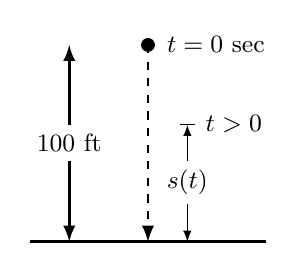
\begin{tikzpicture}[>=latex,every node/.style={font=\small}]
  \draw [line width=1pt,<->] (-1,0) -- (-1,2.5)
   node[midway,fill=white] {$100$ ft};
  \draw [dashed,line width=1pt,->] (0,2.5) -- (0,0)
   node [right,pos=0.0] {$~t=0$ sec};
  \draw [line width=1.2pt] (-1.5,0) -- (1.5,0);
  \fill (0,2.5) circle (2.5pt);
  \draw[<->| ] (0.5,0) -- (0.5,1.5) node [fill=white,midway] {$s(t)$}
   node[right,pos=1.0] {$~t > 0$};
 \end{tikzpicture}}
\par\noindent\emph{Solution:} When the object is dropped at time $t=0$ the only
force acting on it is gravity, causing the object to accelerate downward at the
known constant rate of 32 ft/s\textsuperscript{2}. The object's acceleration
$a(t)$ at time $t$ is thus $a(t) = -32$. If $v(t)$ is the object's velocity at
time $t$, then $v'(t) = a(t)$, which means that\index{straight line motion}
\[
v(t) ~=~ \int a(t)~\dt ~=~ \int -32~\dt ~=~ -32t ~+~ C
\]
for some constant $C$. The constant $C$ here is \emph{not} generic---it has a
specific\\value determined by the \emph{initial condition} on the velocity: the
object was at rest at time $t=0$. That is, $v(0) = 0$, which means
\[
0 ~=~ v(0) ~=~ -32(0) ~+~ C ~=~ C \quad\Rightarrow\quad v(t) ~=~ -32t
\]
for all $t \ge 0$. Likewise, since $s'(t) = v(t)$ then\index{free fall formulas}
\[
s(t) ~=~ \int v(t)~\dt ~=~ \int -32t~\dt ~=~ -16t^2 ~+~ C
\]
for some constant $C$, determined by the initial condition that the object was 
100 ft above the ground at time $t=0$. That is, $s(0) = 100$, which means
\[
100 ~=~ s(0) ~=~ -16(0)^2 ~+~ C ~=~ C \quad\Rightarrow\quad s(t) ~=~ -16t^2 ~+~ 100
\]
for all $t \ge 0$.\quad\checkmark
\end{exmp}\vspace{-2mm}
\divider
\vspace{2mm}

The formula for $s(t)$ in Example \ref{exmp:gravity} can be generalized as
follows: denote the object's initial position at time $t=0$ by $s_0$,
let $v_0$ be the object's initial velocity (positive if thrown upward,
negative if thrown downward), and let $g$ represent the (positive) constant
acceleration due to gravity. By Newton's First Law of motion the only
acceleration imparted to the object \emph{after} throwing it is due to gravity:
\[
a(t) ~=~ -g \quad\Rightarrow\quad v(t) ~=~ \int a(t)~\dt ~=~ \int -g~\dt
~=~ -gt ~+~ C
\]
for some constant $C$:
$v_0 = v(0) = -g \cdot 0 + C = C$. Thus, $v(t) = -gt + v_0$ for all $t \ge 0$,
and so
\[
s(t) ~=~ \int v(t)~\dt ~=~ \int \left(-gt ~+~ v_0\right)~\dt ~=~
-\tfrac{1}{2}gt^2 ~+~ v_0t ~+~ C
\]
for some constant $C$:
$s_0 = s(0) = -\tfrac{1}{2}g \cdot 0^2 + v_0 \cdot 0 + C = C$. To summarize:

\statethm{thm:gravity}{\textbf{Free fall motion:} At time $t \ge 0$:
\begin{alignat*}{3}
\text{acceleration}&\text{:}\quad a(t) ~&&=~ -g\\[4pt]
\text{velocity}&\text{:}\quad v(t) ~&&=~ -gt ~+~ v_0\\[4pt]
\text{position}&\text{:}\quad s(t) ~&&=~ -\tfrac{1}{2}gt^2 ~+~ v_0t ~+~ s_0\\[4pt]
\text{initial conditions}&\text{:}\qquad s_0 ~&&=~ s(0)\,,~v_0 ~=~ v(0)
\end{alignat*}
}
Note that the units are not specified---they just need to be
consistent. In metric units, $g = 9.8 $ m/s\textsuperscript{2}, while
$g = 32 $ ft/s\textsuperscript{2} in English units.\index{free fall formulas}

Thinking of the indefinite integral of a function as the sum of all the
infinitesimal ``pieces'' of that function---for the purpose of retrieving that
function---provides a handy way of integrating a differential equation to obtain
the solution. The key idea is to transform the differential equation into an
\emph{equation of differentials}, which has the effect of treating functions as
variables. Some examples will illustrate the technique.

\begin{exmp}\label{exmp:intdecay}
\noindent For any constant $k$, show that every solution of the differential
equation $\dydt = ky$ is of the form $y = Ae^{kt}$ for some constant
$A$. You can assume that $y(t) > 0$ for all $t$.\vspace{1mm}
\par\noindent\emph{Solution:} Put the $y$ terms on the left and the $t$ terms on
the right, i.e. separate the variables:
\[
\frac{\dy}{y} ~=~ k\,\dt
\]
Now integrate both sides (notice how the \emph{function} $y$ is treated as a
\emph{variable}):
\begin{align*}
\int\,\frac{\dy}{y} ~&=~ \int k\,\dt\\[6pt]
\ln\,y  + C_1 ~&=~ kt + C_2 \quad\text{($C_1$ and $C_2$ are constants)}\\
\ln\,y  ~&=~ kt + C \quad\text{(combine $C_1$ and $C_2$ into the constant $C$)}\\
y ~&=~ e^{kt+C} ~=~ e^{kt} \cdot e^C ~=~ A e^{kt}
\end{align*}
where $A = e^C$ is a constant. Note that this is the formula for radioactive
decay from Section 2.3.
\end{exmp}
\begin{exmp}\label{exmp:intidealgas}
\noindent Recall from Section 3.6 the equation of differentials
\[
\dfrac{\dP}{P} ~+~ \dfrac{\dV}{V} ~=~ \dfrac{\dT}{T}
\]
relating the pressure $P$, volume $V$ and temperature $T$ of an ideal gas.
Integrate that equation to obtain the original ideal gas law $PV = RT$, where
$R$ is a constant.
.\vspace{1mm}
\par\noindent\emph{Solution:} Integrating both sides of the equation yields
\begin{align*}
\int\,\dfrac{\dP}{P} ~+~ \int\,\dfrac{\dV}{V} ~&=~ \int\,\dfrac{\dT}{T}\\[6pt]
\ln\,P ~+~ \ln\,V ~&=~ \ln\,T ~+~ C \quad\text{($C$ is a constant)}\\
\ln\,(PV) ~&=~ \ln\,T ~+~ C\\
PV ~&=~ e^{\ln\,T + C} ~=~ e^{\ln\,T} \cdot e^{C} ~=~ T\,e^C ~=~ RT
\end{align*}
where $R = e^C$ is a constant.\quad\checkmark
\end{exmp}\vspace{-1mm}
\divider
\vspace{2mm}

The integration formulas in this section depended on already knowing the
derivatives of certain functions and then ``working backward'' from their
derivatives to obtain the original functions. Without that prior knowledge you
would be reduced to guessing, or perhaps recognizing a pattern from some
derivative you have encountered. A number of integration techniques will be
presented shortly, but there are many indefinite integrals for which no simple
closed form exists (e.g. $\int e^{x^2}\,\dx$ and
$\int \sin(x^2)\,\dx$).\vspace{2mm}

\divider
\vspace{3mm}
\startexercises\label{sec5dot1}
{\small
\probs{A}
\par\noindent For Exercises 1-15, evaluate the given indefinite integral.
\begin{enumerate}[\bfseries 1.]
\begin{multicols}{3}
 \item $\displaystyle\int\,\left(x^2 ~+~ 5x ~-~ 3\right)~\dx$
 \item $\displaystyle\int\,3 \cos\,x~\dx$
 \item $\displaystyle\int\,4 e^x~\dx$
\end{multicols}
\begin{multicols}{3}
 \item $\displaystyle\int\,\left(x^5 ~-~ 8x^4 ~-~ 3x^3 ~+~ 1\right)~\dx\vphantom{\dfrac{3e^x}{5}}$
 \item $\displaystyle\int\,5 \sin\,x~\dx\vphantom{\dfrac{3e^x}{5}}$
 \item $\displaystyle\int\,\dfrac{3e^x}{5}~\dx$
\end{multicols}
\begin{multicols}{3}
 \item $\displaystyle\int\,\dfrac{6}{x}~\dx$
 \item $\displaystyle\int\,\dfrac{4}{3x}~\dx$
 \item $\displaystyle\int\,\left(-2 \sqrt{x}\,\right)~\dx\vphantom{\dfrac{6}{x}}$
\end{multicols}
\begin{multicols}{3}
 \item $\displaystyle\int\,\dfrac{1}{3 \sqrt{x}}~\dx$
 \item $\displaystyle\int\,\left(x ~+~ x^{4/3}\right)~\dx$
 \item $\displaystyle\int\,\dfrac{1}{3 \sqrt[3]{x}}~\dx$
\end{multicols}
\begin{multicols}{3}
 \item $\displaystyle\int\,3\sec\,x\;\tan\,x~\dx$
 \item $\displaystyle\int\,5 \sec^2x~\dx$
 \item $\displaystyle\int\,7\csc^2x~\dx$
\end{multicols}
 \item Prove the sum and difference rules for indefinite integrals: 
  $\int (f(x) \pm g(x))\,\dx \;=\; \int f(x)\,\dx \;\pm\; \int g(x)\,\dx$
 \item Integrate both sides of the equation
\[
\frac{\dP}{P} ~+~ \frac{d\!M}{M} ~=~ \frac{\dT}{2T}
\]
to obtain the ideal gas continuity relation: $\dfrac{PM}{\sqrt{T}} = $ constant.
 \item\label{exer:projmax0} Use the free fall motion equation for position to
  show that the maximum height reached by an object launched straight up from
  the ground with an initial velocity $v_0$ is $\frac{v_0^2}{2g}$.
\end{enumerate}
}
\newpage
%Begin Section 5.2
\section{The Definite Integral}
Recall from the last section that the integral sign in the indefinite integral
\[
\int\,f(x)~\dx
\]
represents a summation of the infinitesimals $f(x)\,\dx = d\!F$ for an
antiderivative $F(x)$ of $f(x)$. Why is the term ``indefinite'' used? Because
the summation is indefinite: the $x$ in $f(x)\;\dx$ is defined generically,
meaning ``$x$ in general,'' that is, not for $x$ in a specific range of values.
The same summation over a specific, definite range of values of $x$, say, over
an interval $\ival{a}{b}$, is a different type of
integral:\index{definite integral}\index{integral!definite}

\statedefn{defn:defint}{The \textbf{definite integral} of a function $f(x)$ over
an interval $\ival{a}{b}$ is denoted by
\[
\int_a^b\,f(x)~\dx
\]
and represents the sum of the infinitesimals $f(x)\;\dx$ for all $x$ in
$\ival{a}{b}$.}

An indefinite integral yields a \emph{generic function}, whereas a definite
integral yields either a \emph{number} or a \emph{specific} function. There are
many ways to calculate the specific summation in a definite integral, one of
which is motivated by a geometric interpretation of the infinitesimal
$f(x)\;\dx$ as the area of a rectangle, as in Figure \ref{fig:defint} below:

\begin{figure}[ht]
 \begin{center}
  \begin{tikzpicture}[>=latex,every node/.style={font=\small}]
   \draw[line width=1pt] (1,0) -- (1,2.5);
   \draw[line width=1pt] (9,0) -- (9,2);
   \draw [linecolor,line width=1.5pt] (9,2) to[out=140,in=0] (6,3)
    to[out=180,in=0] (3,2) to[out=180,in=-45] (1,2.5);
   \node [above] at (3.5,2.5) {$y = f(x)$};
   \draw[|<->|] (5.4,0) -- (5.4,2.2) node[right,midway] {$f(x)$};
   \draw[<->|] (5.4,2.2) -- (5.4,2.8) node[right,midway] {$f(x+\dx)-f(x)$};
   \filldraw[linecolor,fill=fillcolor] (4,0) -- (4,2.2) -- (5,2.2) -- (5,0);
   \draw[linecolor,dashed] (5,2.2) -- (5,2.8);
   \draw[<->,black!60,line width=1pt,anchor=base] (0,3.3) node[above] {$y$} |-
    (10,0) node[right] {$x$} node[black,shift={(0,-0.4)}] at (1,0) {$a$}
    node[black,shift={(0,-0.4)}] at (9,0) {$b$}
    node[black,shift={(0,-0.4)}] at (4,0) {$x$}
    node[black,shift={(0,-0.4)}] at (5,0) {$x+\dx$};
   \fill (1,2.5) circle (2.5pt);
   \fill (9,2) circle (2.5pt);
   %\draw[|<->|] (4,-0.8) -- (5,-0.8) node[fill=white,inner xsep=.1em,midway] {$\dx$};
   \draw[|<->|] (4,-0.7) -- (5,-0.7) node[below,midway] {$\dx$};
  \end{tikzpicture}\vspace{-5mm}
 \end{center}
 \caption[]{\quad The infinitesimal $f(x)\;\dx$ as the area of a rectangle}
 \label{fig:defint}
\end{figure}

The shaded rectangle in the above picture has height $f(x)$ and width $\dx$, and
so its area is $f(x)\;\dx$. In fact, it appears that that area is just a little
bit smaller than the area under the curve $y=f(x)$ and above the $x$-axis
between $x$ and $x+\dx$; there is a small gap between the curve and the top of
the rectangle, accounting for the difference in the area. However, the area of
that gap turns out to be zero, as shown below:
\newpage
\begin{figure}[ht]
 \begin{center}
  \begin{tikzpicture}[>=latex,every node/.style={font=\small}]
   \draw[|<->|] (1.9,0) -- (1.9,4) node[right,midway] {$f(x)$};
   \draw[<->|] (1.9,4) -- (1.9,5.25) node[right,midway] {$\df=f(x+\dx)-f(x)$};
   \draw (1.3,4) -- (1.3,4.2) -- (1.5,4.2);
   \draw[linecolor,dashed] (1.5,4) -- (1.5,5.25);
   \filldraw[linecolor,fill=fillcolor] (0,0) -- (0,4) -- (1.5,4) -- (1.5,0) -- cycle;
   \draw[linecolor,line width=1.5pt] (0,4) -- (1.5,5.25) node[black,above left,midway] {$y=f(x)$};
   \fill (0,4) circle (2.5pt);
   \fill (1.5,5.25) circle (2.5pt);
   \node[below] at (0,0) {$x\vphantom{\dx}$};
   \node[below] at (1.5,0) {$x+\dx$};
   \draw[|<->|] (0,-0.7) -- (1.5,-0.7) node[below,midway] {$\dx$};
   \node[left] at (0,4) {$A$};
   \node[above] at (1.5,5.25) {$B$};
   \node[below left] at (1.5,4) {$C$};
  \end{tikzpicture}\vspace{-5mm}
 \end{center}
 \caption[]{\quad Area under the curve $y=f(x)$ over $\ival{x}{x+\dx}$}
 \label{fig:defintinf}
\end{figure}

By the Microstraightness Property, the curve $y=f(x)$ shown in Figure
\ref{fig:defint} is a straight line over the infinitesimal interval
$\ival{x}{x+\dx}$, as shown in Figure \ref{fig:defintinf}.\footnote{The function
$f$ is assumed to be differentiable at $x$, in this case. If not then the points
where $f$ is not differentiable can be excluded without affecting the integral.}
Thus, the part of the area between the curve and the $x$-axis over the interval
$\ival{x}{x+\dx}$ consists of two parts: the area $f(x)\,\dx$ of the shaded
rectangle and the area of the right triangle $\triangle ABC$, both of which are
shown in Figure \ref{fig:defintinf}. However, the area of $\triangle ABC$ is
zero:
\[
\text{Area of }\triangle ABC ~=~ \frac{1}{2}\text{(base)}\times\text{(height)}
 ~=~ \frac{1}{2}(\dx)(\df) ~=~ \frac{1}{2}(\dx)(f'(x)\,\dx) ~=~
\frac{1}{2}f'(x)(\dx)^2 ~=~ 0
\]
The function $f$ shown in Figure \ref{fig:defintinf} is increasing at
$x$, but a similar argument could be made if $f$ were decreasing at $x$.
Hence, the area between the curve $y=f(x)$ and the $x$-axis comes solely from
the rectangles with area $f(x)\,\dx$, as $x$ varies from $a$ to $b$. The sum of
all those rectangular areas, though, equals the definite integral of $f(x)$ over
$\ival{a}{b}$. The definite integral can thus be interpreted as an area:
\index{area under a curve}

\statedefn{defn:area}{For a function $f(x) \ge 0$ over $\ival{a}{b}$, the
\textbf{area under the curve} $y=f(x)$ between
$x=a$ and $x=b$, denoted by $A$, is given by
\[
A ~=~ \int_a^b\,f(x)~\dx
\]
and represents the area of the region $R$ bounded above by
$y=f(x)$, bounded below by the $x$-axis, and bounded on the sides by
$x=a$ and $x=b$ (with $a < b$).
}
\newpage
\begin{figure}[ht]
 \begin{center}
  \begin{tikzpicture}[>=latex,every node/.style={font=\small}]
   \fill [fill=fillcolor] (4.2,1) to[out=140,in=-10] (3,1.5)
    to[out=180,in=0] (2,1) to[out=180,in=-45] (1,1.5) -- (1,0) -- (4.2,0) --
    (4.2,1);
   \draw[line width=1pt] (1,0) -- (1,1.5);
   \draw[line width=1pt] (4.2,0) -- (4.2,1);
   \draw [linecolor,line width=1.5pt] (4.2,1) to[out=140,in=-10] (3,1.5)
    to[out=180,in=0] (2,1) to[out=180,in=-45] (1,1.5);
   \node [above] at (2.5,1.5) {$y = f(x)$};
   \draw[<->,black!60,line width=1pt,anchor=base] (0,2.3) node[above] {$y$} |-
    (5,0) node[right] {$x$} node[black,shift={(0,-0.4)}] at (1,0) {$a$}
    node[black,shift={(0,-0.4)}] at (4.2,0) {$b$};
   \node at (2.6,0.7) {$R$};
   \fill (1,1.5) circle (2.5pt);
   \fill (4.2,1) circle (2.5pt);
  \end{tikzpicture}\vspace{-6mm}
 \end{center}
 \caption[]{\quad The area $A$ of the region $R$ equals $\int_a^bf(x)\,\dx$}
 \label{fig:defintarea}
\end{figure}

In Figure \ref{fig:defintarea} the area under the curve $y=f(x)$ between $x=a$
and $x=b$ is the area $A$ of the shaded region $R$, namely
$A = \int_a^bf(x)\,\dx$. To calculate that area for a specific function,
rectangles can again be used, but this time with widths that are small positive
numbers instead of infinitesimals. The procedure is as follows:
\index{partition}

\begin{enumerate}[\bfseries 1.]
 \item Create a \textbf{partition} $P = \lbrace x_0 < x_1 < \cdots < x_{n-1}
  < x_n \rbrace$ of the interval $\ival{a}{b}$ into $n \ge 1$ subintervals
  $\ival{x_0}{x_1}$, $\ival{x_1}{x_2}$, $\ldots$, $\ival{x_{n-1}}{x_n}$, with
  $x_0 = a$ and $x_n = b$.
 \item In each subinterval $\ival{x_{i-1}}{x_i}$ of $P$ pick a
  number $x_i^*$, so that $x_{i-1} \le x_i^* \le x_i$ for $i=1$ to $n$.
 \item For $i=1$ to $n$, form a rectangle whose base is the subinterval
  $\ival{x_{i-1}}{x_i}$ of length $\Delta x_i = x_i - x_{i-1} > 0$ and whose
  height is $f(x_i^*)$.
 \item Take the sum $f(x_1^*) \Delta x_1 + f(x_2^*) \Delta x_2 + \cdots +
  f(x_n^*) \Delta x_n$ of the areas of these rectangles, called a
  \textbf{Riemann sum}.\index{Riemann sum}

\begin{figure}[ht]
 \begin{center}
  \begin{tikzpicture}[>=latex,every node/.style={font=\small}]
   \draw[line width=1pt] (1,0) -- (1,2.5);
   \draw[line width=1pt] (9,0) -- (9,2);
   \node [above] at (3.5,2.5) {$y = f(x)$};
   \filldraw[linecolor,fill=fillcolor,fill opacity=0.5] (1,0) -- (1,2.2) -- (2,2.2) -- (2,0);
   \filldraw[linecolor,fill=fillcolor,fill opacity=0.5] (2,0) -- (2,2) -- (4,2) -- (4,0);
   \filldraw[linecolor,fill=fillcolor,fill opacity=0.5] (7.5,0) -- (7.5,2.4) -- (9,2.4) -- (9,0);
   \draw [linecolor,line width=1.5pt] (9,2) to[out=140,in=0] (6,3)
    to[out=180,in=0] (3,2) to[out=180,in=-45] (1,2.5);
   \draw[<->,linecolor,dashed] (1.5,0) -- (1.5,2.2)
    node[black,fill=fillcolor,midway,inner xsep=0em,fill opacity=0.5] {$f(x_1^*)$};
   \draw[<->,linecolor,dashed] (2.5,0) -- (2.5,2)
    node[black,fill=fillcolor,midway,inner xsep=0em,fill opacity=0.5] {$f(x_2^*)$};
   \draw[<->,linecolor,dashed] (8.5,0) -- (8.5,2.4)
    node[black,fill=fillcolor,midway,inner xsep=0em,fill opacity=0.5] {$f(x_n^*)$};
   \draw[<->,black!60,line width=1pt,anchor=base] (0,3) node[above] {$y$} |-
    (10.5,0) node[right] {$x$} node[black,shift={(0,-0.4)}] at (1,0) {$x_0$}
    node[black,shift={(0,-0.4)}] at (0.5,0) {$a=$}
    node[black,shift={(0,-0.4)}] at (1.5,0) {$x_1^*$}
    node[black,shift={(0,-0.4)}] at (2,0) {$x_1$}
    node[black,shift={(0,-0.4)}] at (2.5,0) {$x_2^*$}
    node[black,shift={(0,-0.4)}] at (4,0) {$x_2$}
    node[black,shift={(0,-0.4)}] at (5.75,0) {$\ldots$}
    node[black,shift={(0,-0.4)}] at (7.5,0) {$x_{n-1}$}
    node[black,shift={(0,-0.4)}] at (8.5,0) {$x_n^*$}
    node[black,shift={(0,-0.4)}] at (9,0) {$x_n$}
    node[black,shift={(0,-0.4)}] at (9.5,0) {$=b$};
   \node at (5.75,1) {$\ldots$};
   \fill (1,2.5) circle (2.5pt);
   \fill (9,2) circle (2.5pt);
   \draw[|<->|] (1,-0.7) -- (2,-0.7) node[below,midway] {$\Delta x_1$};
   \draw[<->|] (2,-0.7) -- (4,-0.7) node[below,midway] {$\Delta x_2$};
   \draw[|<->|] (7.5,-0.7) -- (9,-0.7) node[below,midway] {$\Delta x_n$};
  \end{tikzpicture}\vspace{-5mm}
 \end{center}
 \caption[]{\quad A Riemann sum of $f(x)$ over a partition of $\ival{a}{b}$}
 \label{fig:riemannsum}
\end{figure}

 \item Take the limit of the Riemann sums as $n \to \infty$, so that the
  subinterval lengths approach 0. If the limit
  exists then that limit is the area $A$ of the region $R$:
\begin{equation}\label{eqn:riemannsum}
\text{Area } A ~=~ \int_a^b\,f(x)~\dx ~=~ \lim_{n \to \infty}~\sum_{i=1}^{n} f(x_i^*)\,\Delta x_i
\end{equation}
\end{enumerate}

The limit in Formula (\ref{eqn:riemannsum}) should be taken over all partitions
whose \textbf{norm}---the length of the largest subinterval---approaches
0\index{norm of a partition}\index{partition!norm}. In practice,
however, the partitions are usually chosen so that the subintervals are of equal
length, and then simply make those equal lengths smaller and smaller by
dividing the interval $\ival{a}{b}$ into more and more such subintervals.
Note that the points $x_i^*$ in each subinterval can be anywhere in the
subinterval---often the midpoint of the subinterval is
chosen, but the left and right endpoints are also typical choices.

In the above procedure the gaps between the rectangles and the curve will have
areas approaching 0 as the number $n$ of subintervals grows and the
subinterval lengths approach 0. This is true if the function $f$ is
differentiable, and in fact even if $f$ is merely continuous.\footnote{For a
proof and fuller discussion of all this, see Ch.1-2 in \textsc{Knopp, M.I.},
\emph{Theory of Area}, Chicago: Markham Publishing Co., 1969. The book
attempts to define precisely what an ``area'' actually means, including
that of a rectangle (showing agreement with the intuitive notion of width times
height).} Thus, the area under the curve can be \emph{defined} by the above
procedure. 

To calculate the area under a curve in this manner, the reader should have some
familiarity with the summation notation in Formula (\ref{eqn:riemannsum}).

\statedefn{defn:summation}{For real numbers $a_1$, $a_2$, $\ldots$, $a_n$ and
an integer $n \ge 1$,
\[
\sum_{k=1}^{n} a_k ~=~ a_1 ~+~ a_2 ~+~ \cdots ~+~ a_n
\]
is the sum of $a_1$, $\ldots$, $a_n$. The symbol $\Sigma$ is called the
\textbf{summation sign}, which is the Greek capital letter
Sigma.\index{sigma notation}}

The following rules for this ``Sigma notation'' are intuitively obvious:

\statethm{thm:sigmarules}{Let $a_1$, $a_2$, $\ldots$, $a_n$, and
$b_1$, $b_2$, $\ldots$, $b_n$ be real numbers, and let $c$ be a constant.
Then:\vspace{2mm}
\begin{enumerate}[\bfseries (1)]
 \item $\displaystyle\sum_{k=1}^{n} (a_k + b_k) ~=~
\displaystyle\sum_{k=1}^{n} a_k ~+~ \displaystyle\sum_{k=1}^{n} b_k$
 \item $\displaystyle\sum_{k=1}^{n} (a_k - b_k) ~=~
\displaystyle\sum_{k=1}^{n} a_k ~-~ \displaystyle\sum_{k=1}^{n} b_k$
 \item $\displaystyle\sum_{k=1}^{n} c a_k ~=~ c\,\displaystyle\sum_{k=1}^{n} a_k$
 \item $\displaystyle\sum_{k=1}^{n} a_k ~=~ \displaystyle\sum_{i=1}^{n} a_i$
 \quad (i.e. the sum is independent of the summation index letter)
\end{enumerate}
}
\newpage
\noindent The following summation formulas can be helpful when calculating
Riemann sums:

\statethm{thm:sumformulas}{Let $n \ge 1$ be a positive integer.
Then:\vspace{2mm}
\begin{enumerate}[\bfseries (1)]
 \item $\displaystyle\sum_{k=1}^{n} 1 ~=~ n$
 \item $\displaystyle\sum_{k=1}^{n} k ~=~ 1 ~+~ 2 ~+~ \cdots ~+~ n ~=~ 
  \dfrac{n\,(n + 1)}{2}$
 \item $\displaystyle\sum_{k=1}^{n} k^2 ~=~ 1^2 ~+~ 2^2 ~+~ \cdots ~+~ n^2 ~=~ 
  \dfrac{n\,(n + 1)\,(2n + 1)}{6}$
 \item $\displaystyle\sum_{k=1}^{n} k^3 ~=~ 1^3 ~+~ 2^3 ~+~ \cdots ~+~ n^3 ~=~ 
  \dfrac{n^2\,(n + 1)^2}{4}$
 \item $\displaystyle\sum_{k=1}^{n} k^4 ~=~ 1^4 ~+~ 2^4 ~+~ \cdots ~+~ n^4 ~=~ 
  \dfrac{n\,(n + 1)\,(6n^3 + 9n^2 + n - 1)}{30}$
\end{enumerate}
}

\noindent Formula (1) is obvious: add the number $1$ a total of $n$ times and
the sum is $n$.\\Formula (2) can be proved by induction:

\begin{enumerate}
 \item Show that $\displaystyle\sum_{k=1}^{n} k ~=~ \dfrac{n\,(n + 1)}{2}$ for
 $n=1$:
\[
\sum_{k=1}^{1} k ~=~ 1 ~=~ \frac{1\,(1 + 1)}{2} \quad\checkmark
\]
 \item Assume that $\displaystyle\sum_{k=1}^{n} k ~=~ \dfrac{n\,(n + 1)}{2}$ for
 some integer $n \ge 1$. Show that the formula holds for $n$ replaced by $n+1$,
 that is:
\[
\sum_{k=1}^{n+1} k ~=~ \frac{(n + 1)\,((n + 1) + 1)}{2} ~=~
\frac{(n + 1)\,(n + 2)}{2}
\]
To show this, note that
\begin{align*}
 \sum_{k=1}^{n+1} k ~&=~ 1 ~+~ 2 ~+~ \cdots ~+~ n ~+~ (n+1)
  ~=~ \sum_{k=1}^{n} k ~+~ (n+1)\\[6pt]
&=~ \frac{n\,(n + 1)}{2} ~+~ (n+1) ~=~ \frac{n\,(n + 1) ~+~ 2(n+1)}{2} ~=~
\frac{(n + 1)\,(n + 2)}{2} \quad\checkmark
\end{align*}
 \item By induction, this proves the formula for all integers $n \ge 1$.
\quad\qedsymbol
\end{enumerate}
\newpage
\noindent Formulas (3)-(5) can be proved similarly by induction (see the
exercises). The example below shows how Formulas (2) and (3) are used in finding
the limit of a Riemann sum.

\begin{exmp}\label{exmp:riemann1}
\noindent Use Riemann sums to calculate
$\displaystyle\int_1^2 x^2~\dx$.\vspace{1mm}
\par\noindent\emph{Solution:} The definite integral is the area under the curve
$y=f(x)=x^2$ between $x=1$ and $x=2$, as shown in Figure \ref{fig:riemann1}(a):

\begin{figure}[ht]
 \centering
 \subfloat[][ Area under $y=x^2$ over $\ival{1}{2}$]{
 \begin{tikzpicture}[>=latex,every node/.style={font=\small}]
  \node[below left] at (0,0) {$0$};
  \fill[fillcolor] (1,0) -- (1,0.5) parabola (4,4) -- (4,0);
  \draw[linecolor,line width=1.5pt] (1,0.5) parabola (4,4);
  \draw[linecolor,line width=1pt] (1,0) -- (1,0.5);
  \draw[linecolor,line width=1pt] (4,0) -- (4,4);
  \draw [<->,black!60,line width=1pt,anchor=base] (0,4) node[above] {$y$}
   |- (5.5,0) node[right] {$x$}
  node[black,shift={(0,-0.4)}] at (1,0) {$1$}
  node[black,shift={(0,-0.4)}] at (4,0) {$2$};
  \fill (1,0.5) circle (2.5pt);
  \fill (4,4) circle (2.5pt);
 \end{tikzpicture}}
 \qquad\quad
 \subfloat[][ Riemann sums using left endpoints: $x_i^*=x_{i-1}$]{
 \begin{tikzpicture}[>=latex,every node/.style={font=\small}]
  \node[below left] at (0,0) {$0$};
  \draw[linecolor,line width=1.5pt] (1,0.5) parabola (4,4);
  \filldraw[linecolor,fill=fillcolor,line width=1pt] (1,0) -- (1,0.5) -- (1.5,0.5) -- (1.5,0);
  \filldraw[linecolor,fill=fillcolor,line width=1pt] (1.5,0) -- (1.5,0.5972) -- (2,0.5972) -- (2,0);
  \filldraw[linecolor,fill=fillcolor,line width=1pt] (3.5,0) -- (3.5,2.9305) -- (4,2.9305) -- (4,0);
  \draw[linecolor,line width=1pt] (4,0) -- (4,4);
  \draw [<->,black!60,line width=1pt,anchor=base] (0,4) node[above] {$y$}
   |- (6.5,0) node[right] {$x$}
  node[black,shift={(0,-0.4)}] at (0.5,0) {$1=$}
  node[black,shift={(0,-0.4)}] at (1,0) {$x_0$}
  node[black,shift={(0,-0.4)}] at (1.5,0) {$x_1$}
  node[black,shift={(0,-0.4)}] at (2,0) {$x_2$}
  node[black,shift={(0,-0.4)}] at (2.75,0) {$\ldots$}
  node[black,shift={(0,-0.4)}] at (3.4,0) {$x_{n-1}$}
  node[black,shift={(0,-0.4)}] at (4,0) {$x_n$}
  node[black,shift={(0,-0.4)}] at (4.5,0) {$=2$};
  \fill (1,0.5) circle (2.5pt);
  \fill (4,4) circle (2.5pt);
  \node at (2.75,0.8) {$\ldots$};
 \end{tikzpicture}}
 \caption[]{\quad Calculating $\int_1^2 x^2~\dx$}
 \label{fig:riemann1}
\end{figure}

\noindent Divide the interval $\ival{1}{2}$ into $n$ subintervals of equal
length $\Delta x_i = (2-1)/n = 1/n$ for $i =1$ to $n$, so that the partition $P$ is
$\lbrace x_0 < x_1 < \ldots x_n \rbrace$ where $x_i = 1 + \frac{i}{n}$ for
$i=0$, $1$, $\ldots$, $n$ (and hence $x_0=1$ and $x_n=2$). In each subinterval
$\ival{x_{i-1}}{x_i}$ pick the point $x_i^*$ to be the left endpoint $x_{i-1}$,
so that the rectangles appear as in Figure \ref{fig:riemann1}(b). Then
\begin{align*}
\int_1^2 x^2~\dx ~&=~ \lim_{n \to \infty}~\sum_{i=1}^{n} f(x_i^*)\,\Delta x_i
~=~ \lim_{n \to \infty}~\sum_{i=1}^{n} f(x_{i-1})\,\frac{1}{n}
~=~ \lim_{n \to \infty}~\sum_{i=1}^{n} x_{i-1}^2\,\frac{1}{n}\\[6pt]
&=~ \lim_{n \to \infty}~\sum_{i=1}^{n} \left(1 + \frac{i-1}{n}\right)^2\frac{1}{n}
~=~ \lim_{n \to \infty}~\sum_{i=1}^{n} \left(\frac{1}{n} ~+~ \frac{2}{n^2}(i-1) ~+~
 \frac{1}{n^3}(i-1)^2\right)\\[6pt]
&=~ \lim_{n \to \infty}~\left(\sum_{i=1}^{n}\frac{1}{n} ~+~ \frac{2}{n^2}\sum_{i=1}^{n}(i-1) ~+~
    \frac{1}{n^3}\sum_{i=1}^{n}(i-1)^2\right)
~=~ \lim_{n \to \infty}~\left(1 ~+~ \frac{2}{n^2}\sum_{i=1}^{n-1}i ~+~
    \frac{1}{n^3}\sum_{i=1}^{n-1}i^2\right)\\[6pt]
&= \lim_{n \to \infty}~\left(1 \;+\; \frac{2}{n^2}\cdot\frac{(n-1)n}{2} \;+\;
   \frac{1}{n^3}\cdot\frac{(n-1)n(2n-1)}{6}\right)\quad\text{(replace $n$ by $n-1$ in Formulas (2) and (3))}\\[6pt]
&=~ \left(\lim_{n \to \infty}\,1\right) ~+~ \left(\lim_{n \to \infty}\,\frac{n-1}{n}\right)
    ~+~ \left(\lim_{n \to \infty}\,\frac{2n^2-3n+1}{6n^2}\right)\\[6pt]
&=~ 1 ~+~ \frac{1}{1} ~+~ \frac{2}{6} ~=~ \frac{7}{3}
\end{align*}
\end{exmp}
\divider
\newpage
It it often simpler to use a computer to calculate approximations of a definite
integral, by taking the Riemann sum of a sufficiently large number of
rectangles in order to achieve the desired accuracy. Choosing subintervals of
equal length, as in Example \ref{exmp:riemann1}, makes it easier to use an
algorithm to calculate the integral.

For example, the table below summarizes the calculations of Riemann sums for the
function in Example \ref{exmp:riemann1}---namely $f(x)= x^2$ over
$\ival{1}{2}$---using different values for the points $x_i^*$ in the
subintervals (left endpoints, midpoints, and right endpoints):

\begin{center}
\texttt\small{
 \begin{tabular}{|l|l|l|l|}
  \hline
  \rowcolor{fillcolor} \# of rectangles & Left endpoint & Midpoint & Right endpoint\\
  \hline
  1 & 1 & 2.25 & 4\\
  \hline
  2 & 1.625 & 2.3125 & 3.125\\
  \hline
  3 & 1.851851851852 & 2.324074074074 & 2.851851851852\\
  \hline
  4 & 1.96875 & 2.328125 & 2.71875\\
  \hline
  5 & 2.04 & 2.33 & 2.64\\
  \hline
  10 & 2.185 & 2.3325 & 2.485\\
  \hline
  % 50 & 2.3034 & 2.3333 & 2.3634\\
  % \hline
  100 & 2.31835 & 2.333325 & 2.34835\\
  \hline
  % 500 & 2.330334 & 2.333333 & 2.336334\\
  % \hline
  1000 & 2.3318335 & 2.33333325 & 2.3348335\\
  \hline
  10000 & 2.333183335 & 2.3333333325 & 2.333483335\\
  \hline
  100000 & 2.33331833335 & 2.333333333325 & 2.33334833335\\
  \hline
  1000000 & 2.333331833333 & 2.333333333333 & 2.333334833333\\
  \hline
 \end{tabular}}
\end{center}\vspace{-2mm}

Due to the concavity of the curve $y=x^2$, using the left endpoints
underestimates the actual area, whereas using the right endpoints yields an
overestimate. Using the midpoints usually gives better results (i.e. more
accuracy in fewer iterations).

So far only definite integrals of nonnegative functions have been
considered---that is, functions $f(x) \ge 0$ over an interval $\ival{a}{b}$. If
$f(x)$ is either negative or changes sign over $\ival{a}{b}$, then the definite
integral can be defined as follows:

\statedefn{defn:defintneg}{Let $R$ be the region bounded by $y=f(x)$ and the
$x$-axis between $x=a$ and $x=b$. If $f(x) \le 0$ over $\ival{a}{b}$, then
\[
\int_a^b\,f(x)~\dx ~=~ \text{the negative of the area of $R$}
\]
If $f(x)$ changes sign over $\ival{a}{b}$, then
\[
\int_a^b\,f(x)~\dx ~=~ \text{the net area of $R$,}
\]
where the parts of $R$ above the $x$-axis count as positive area and the parts
below count as negative area.
}
\newpage
\noindent Note: In the definite integral $\displaystyle\int_a^b\,f(x)\;\dx$
the numbers $a$ and $b$ are called the
\textbf{limits of integration}\index{limits of integration}, with $a$ being the
\textbf{lower limit of integration} and $b$ the \textbf{upper limit of
integration}. The function $f(x)$ being integrated is called the
\textbf{integrand}\index{integrand}, in both definite and indefinite
integrals.\vspace{2mm}

\divider
\vspace{2mm}
\startexercises\label{sec5dot2}
{\small
\probs{A}
\begin{enumerate}[\bfseries 1.]
 \item Explain why $\displaystyle\int_a^b c~\dx ~=~ c(b-a)$ for any constant $c$.
 \item Would using left endpoints in the Riemann sums underestimate or overestimate
 $\int_1^2 \ln x\,\dx$? Explain.
\suspend{enumerate}
\probs{B}
\resume{enumerate}[{[\bfseries 1.]}]
\begin{multicols}{2}
 \item Use Riemann sums to calculate $\displaystyle\int_0^1 x~\dx$.
 \item Use Riemann sums to calculate $\displaystyle\int_0^1 x^2~\dx$.
\end{multicols}
\begin{multicols}{2}
 \item Use Riemann sums to calculate $\displaystyle\int_0^1 3x^2~\dx$.
 \item Use Riemann sums to calculate $\displaystyle\int_0^1 x^3~\dx$.
\end{multicols}
 \item Prove the formula $~\displaystyle\sum_{k=1}^{n}~k^2 ~=~ \dfrac{n\,(n+1)\,(2n+1)}{6}~$
 by induction on $n\ge 1$.
 \item Prove the formula $~\displaystyle\sum_{k=1}^{n}~k^2 ~=~ \dfrac{n\,(n+1)\,(2n+1)}{6}~$ as follows:
  \begin{enumerate}[\bfseries (a)]
   \item Show that $~\displaystyle\sum_{k=1}^{n}~\left( (k+1)^3 ~-~ k^3 \right) ~=~ (n+1)^3 ~-~ 1~$.
   \item Show that $(k+1)^3 ~-~ k^3 ~=~ 3k^2 ~+~ 3k ~+~ 1~$.
   \item Use the formula $~\displaystyle\sum_{k=1}^{n}~k ~=~ \dfrac{n\,(n+1)}{2}~$ and parts (a) and (b)
    to show that $~\displaystyle\sum_{k=1}^{n}~k^2 ~=~ \dfrac{n\,(n+1)\,(2n+1)}{6}~$.
  \end{enumerate}
 \item Prove the formula $~\displaystyle\sum_{k=1}^{n}~k^3 ~=~
  \dfrac{n^2\,(n+1)^2}{4}~$ by induction on $n \ge 1$.
 \item The famous \emph{quicksort algorithm} in computer science is a popular
method for placing objects in some order (e.g. numerical, alphabetical). On average
the algorithm needs $O(n\;\log\,n)$ comparisons to sort $n$ objects (here $\log\,n$
means the natural logarithm of $n$). The proof of that average \emph{complexity}
depends on the inequality\index{quicksort algorithm}
\[
 \sum_{k=2}^{m-1}\;k\,\ln\,k ~\le~ \int_2^m x\,\ln\,x\;\dx
\]
for all integers $m > 2$. Explain why that inequality is true.
\suspend{enumerate}
\probs{C}
\resume{enumerate}[{[\bfseries 1.]}]
 \item Prove the formula $\displaystyle\sum_{k=1}^{n} k^4 ~=~ 1^4 ~+~ 2^4 ~+~
  \cdots ~+~ n^4 ~=~ \dfrac{n\,(n + 1)\,(6n^3 + 9n^2 + n - 1)}{30}$ by induction on
  $n \ge 1$.
 \item Calculate the following sum:
\[
1 ~+~ (1 + 2) ~+~ (1 + 2 + 3) ~+~ (1 + 2 + 3 + 4) ~+~ \cdots ~+~
(1 + 2 + 3 + 4 + \cdots + 50)
\]
\end{enumerate}
}
\newpage
%Begin Section 5.3
\section{The Fundamental Theorem of Calculus}
Using Riemann sums to calculate definite integrals can be tedious, as was seen
in the previous section. In fact the technique shown in that section depended on
the function being a low-degree polynomial, which obviously will not always be
the case. Luckily there is a better way, involving antiderivatives, given by the
following theorem:\index{Fundamental Theorem of Calculus}

\statethm{thm:ftc}{\textbf{Fundamental Theorem of Calculus}:
Suppose that a function $f$ is differentiable on $\ival{a}{b}$.
Then:\vspace{2mm}
\begin{enumerate}[\bfseries (I)]
 \item The function $A(x)$ defined on $\ival{a}{b}$ by
 \[
  A(x) ~=~ \int_a^x\,f(t)~\dt
 \]
 is differentiable on $\ival{a}{b}$, and
 \[
  A'(x) ~=~ f(x)
 \]
 for all $x$ in $\ival{a}{b}$.
 \item If $F$ is an antiderivative of $f$ on $\ival{a}{b}$, i.e. $F'(x) = f(x)$
  for all $x$ in $\ival{a}{b}$, then
 \[
  \int_a^b\,f(x)~\dx ~=~ F(b) ~-~ F(a) ~.
 \]
\end{enumerate}
}

The function $A(x)$ in Part I of the theorem is sometimes called the
\textbf{area function}\index{area function}\index{function!area} because
it represents the area under the curve $y=f(x)$ over the interval $\ival{a}{x}$,
as shown in Figure \ref{fig:ftc1} below.

\begin{figure}[ht]
\begin{minipage}[b]{7.5cm}
 \begin{center}
  \begin{tikzpicture}[>=latex,every node/.style={font=\small}]
   \fill [fill=fillcolor] (3,1.5)
    to[out=180,in=0] (2,1) to[out=180,in=-45] (1,1.5) -- (1,0) -- (3,0) --
    (3,1.5);
   \draw[line width=1pt] (1,0) -- (1,1.5);
   \draw[line width=1pt] (3,0) -- (3,1.5);
   \draw [linecolor,line width=1.5pt] (4.2,1) to[out=140,in=-10] (3,1.5)
    to[out=180,in=0] (2,1) to[out=180,in=-45] (1,1.5);
   \node [above] at (2.5,1.5) {$y = f(x)$};
   \draw[<->,black!60,line width=1pt,anchor=base] (0,2.3) node[above] {$y$} |-
    (5,0) node[right] {$x$} node[black,shift={(0,-0.4)}] at (1,0) {$a$}
    node[black,shift={(0,-0.4)}] at (3,0) {$x$}
    node[black,shift={(0,-0.4)}] at (4.2,0) {$b$};
   \node at (2,0.5) {$A(x)$};
   \fill (1,1.5) circle (2.5pt);
   \fill (4.2,1) circle (2.5pt);
  \end{tikzpicture}\vspace{-6mm}
 \end{center}
 \caption[]{\quad The area function $A(x) = \int_a^xf(t)\,\dt$}
 \label{fig:ftc1}
\end{minipage}
\begin{minipage}[b]{7.5cm}
 \begin{center}
  \begin{tikzpicture}[>=latex,every node/.style={font=\small}]
   \fill [fill=fillcolor] (3,1.5)
    to[out=180,in=0] (2,1) -- (2,0) -- (3,0) -- (3,1.5);
   \draw[line width=1pt] (2,0) -- (2,1);
   \draw[line width=1pt] (3,0) -- (3,1.5);
   \draw [linecolor,line width=1.5pt] (4.2,1) to[out=140,in=-10] (3,1.5)
    to[out=180,in=0] (2,1) to[out=180,in=-45] (1,1.5);
   \node [above] at (2.5,1.5) {$y = f(x)$};
   \draw[<->,black!60,line width=1pt,anchor=base] (0,2.3) node[above] {$y$} |-
    (5,0) node[right] {$x$} node[black,shift={(0,-0.4)}] at (1,0) {$a$}
    node[black,shift={(0,-0.4)}] at (2,0) {$x$}
    node[black,shift={(0,-0.4)}] at (3,0) {$x+\dx$}
    node[black,shift={(0,-0.4)}] at (4.2,0) {$b$};
   \node at (2.5,0.5) {$\dA$};
   \fill (1,1.5) circle (2.5pt);
   \fill (4.2,1) circle (2.5pt);
  \end{tikzpicture}\vspace{-6mm}
 \end{center}
 \caption[]{\quad $\dA = A(x+\dx) - A(x)$}
 \label{fig:ftc1dA}
\end{minipage}
\end{figure}\vspace{-2mm}

To prove Part I, assume that $f(x) \ge 0$ on $\ival{a}{b}$ as in Figure
\ref{fig:ftc1} (the proofs for $f(x)$ either negative or
switching sign over $\ival{a}{b}$ are similar). The goal is to show that for any
$x$ in $\ival{a}{b}$ the differential $\dA$ exists and equals $f(x)\,\dx$.
First, $\dA = A(x+\dx) - A(x)$ is the area under the curve $y=f(x)$ over the
interval $\ival{x}{x+\dx}$, as shown in Figure \ref{fig:ftc1dA} above.
\newpage
By the Microstraightness Property the curve $y=f(x)$ is a straight line over the
infinitesimal
interval $\ival{x}{x+\dx}$, so $f$ must be either increasing, constant, or
decreasing over that interval. The three possibilities are shown in Figure
\ref{fig:ftc1dA3}:

\begin{figure}[ht]
 \centering
 \subfloat[][ $f$ is increasing]{
 \begin{tikzpicture}[>=latex,every node/.style={font=\small}]
   \draw[|<->|] (-0.4,0) -- (-0.4,4) node[left,midway] {$f(x)$};
   \draw[|<->|] (1.9,0) -- (1.9,4) node[right,midway] {$f(x)$};
   \draw[<->|] (1.9,4) -- (1.9,5.25) node[right,midway] {$\df$};
   \filldraw[linecolor,fill=fillcolor] (0,0) -- (0,4) -- (1.5,5.25) -- (1.5,0) -- cycle;
   \draw[linecolor,dashed] (0,4) -- (1.5,4);
   \draw[linecolor] (1.3,4) -- (1.3,4.2) -- (1.5,4.2);
   \draw[linecolor,line width=1.5pt] (0,4) -- (1.5,5.25) node[black,above left,midway] {$y=f(x)$};
   \fill (0,4) circle (2.5pt);
   \fill (1.5,5.25) circle (2.5pt);
   \node[below] at (0,0) {$x\vphantom{\dx}$};
   \node[below] at (1.5,0) {$x+\dx$};
   \draw[|<->|] (0,-0.7) -- (1.5,-0.7) node[below,midway] {$\dx$};
   \node[above] at (0,4) {$A$};
   \node[above] at (1.5,5.25) {$B$};
   \node[below left] at (1.5,4) {$C$};
 \end{tikzpicture}}
 \qquad
 \subfloat[][ $f$ is constant]{
 \begin{tikzpicture}[>=latex,every node/.style={font=\small}]
   \draw[|<->|] (-0.4,0) -- (-0.4,4) node[left,midway] {$f(x)$};
   \filldraw[linecolor,fill=fillcolor] (0,0) -- (0,4) -- (1.5,4) -- (1.5,0) -- cycle;
   \draw[linecolor,line width=1.5pt] (0,4) -- (1.5,4) node[black,above,midway] {$y=f(x)$};
   \fill (0,4) circle (2.5pt);
   \fill (1.5,4) circle (2.5pt);
   \node[below] at (0,0) {$x\vphantom{\dx}$};
   \node[below] at (1.5,0) {$x+\dx$};
   \draw[|<->|] (0,-0.7) -- (1.5,-0.7) node[below,midway] {$\dx$};
 \end{tikzpicture}}
 \qquad
 \subfloat[][ $f$ is decreasing]{
 \begin{tikzpicture}[>=latex,every node/.style={font=\small}]
   \draw[|<->|] (-0.4,0) -- (-0.4,5.25) node[left,midway] {$f(x)$};
   \draw[|<->|] (1.9,0) -- (1.9,4) node[right,midway] {$f(x+\dx)$};
   \draw[<->|] (1.9,4) -- (1.9,5.25) node[right,midway] {$-\df$};
   \filldraw[linecolor,fill=fillcolor] (0,0) -- (0,5.25) -- (1.5,4) -- (1.5,0) -- cycle;
   \draw[linecolor,dashed] (0,4) -- (1.5,4);
   \draw[linecolor] (0.2,4) -- (0.2,4.2) -- (0,4.2);
   \draw[linecolor,line width=1.5pt] (0,5.25) -- (1.5,4) node[black,above right,pos=0.2] {$y=f(x)$};
   \fill (0,5.25) circle (2.5pt);
   \fill (1.5,4) circle (2.5pt);
   \node[below] at (0,0) {$x\vphantom{\dx}$};
   \node[below] at (1.5,0) {$x+\dx$};
   \draw[|<->|] (0,-0.7) -- (1.5,-0.7) node[below,midway] {$\dx$};
   \node[above] at (0,5.25) {$A$};
   \node[above] at (1.5,4) {$B$};
   \node[below right] at (0,4) {$C$};
 \end{tikzpicture}}
 \caption[]{\quad The three possibilities for $\dA$}
 \label{fig:ftc1dA3}
\end{figure}

In the case where $f$ is increasing over $\ival{x}{x+\dx}$, the infinitesimal
area $\dA$ is the sum of the area of the rectangle of height $f(x)$ and width
$\dx$ and the area of the right triangle $\triangle ABC$ shown in Figure
\ref{fig:ftc1dA3}(a). The area of $\triangle ABC$ is $\frac{1}{2}(\df)(\dx)
= \frac{1}{2}f'(x)(\dx)^2 = 0$, so $\dA = f(x)\,\dx$.

In the case where $f$ is constant over $\ival{x}{x+\dx}$, the infinitesimal
area $\dA$ is the area of the rectangle of height $f(x)$ and width $\dx$, as
shown in Figure \ref{fig:ftc1dA3}(b). So again, $\dA = f(x)\,\dx$.

In the case where $f$ is decreasing over $\ival{x}{x+\dx}$, the infinitesimal
area $\dA$ is the sum of the area of the rectangle of height $f(x+\dx)$ and
width $\dx$ and the area of the right triangle $\triangle ABC$ shown in Figure
\ref{fig:ftc1dA3}(c). Note that $\df < 0$ since $f$ is decreasing, and so the
area of $\triangle ABC$ is $\frac{1}{2}(-\df)(\dx) = -\frac{1}{2}f'(x)(\dx)^2
= 0$. Thus,
\[
\dA ~=~ f(x+\dx)\,\dx ~=~ (f(x) + \df)\,\dx ~=~
        f(x)\,\dx ~+~ f'(x)(\dx)^2 ~=~ f(x)\,\dx ~+~ 0 ~=~ f(x)\,\dx ~.
\]

So in all three cases, $\dA = f(x)\,\dx$, and so $A'(x) = \frac{\dA}{\dx} = f(x)$,
which shows that $A(x)$ is differentiable and has derivative $f(x)$.
This proves Part I of the Fundamental Theorem of Calculus.$\quad\checkmark$

To prove Part II of the theorem, let $F(x)$ be an antiderivative of $f(x)$ over
$\ival{a}{b}$. Since the area function $A(x) = \int_a^x f(x)\,\dx$ is also an
antiderivative of
$f(x)$ over $\ival{a}{b}$ by Part I of the theorem, then $A(x)$ and $F(x)$
differ by a constant $C$ over $\ival{a}{b}$. In other words:

\[
 A(x) ~=~ F(x) ~+~ C \quad\text{for all $x$ in $\ival{a}{b}$}
\]
\newpage
By definition $A(a) = 0$, since it is the area under the curve over the
interval $\ival{a}{a}$ of zero length. Thus,
\[
0 ~=~ A(a) ~=~ F(a) ~+~ C \quad\Rightarrow\quad C ~=~ -F(a)
\quad\Rightarrow\quad A(x) ~=~ F(x) ~-~ F(a)
\quad\text{for all $x$ in $\ival{a}{b}$}
\]
and so
\[
\int_a^b f(x)~\dx ~=~ A(b) ~=~ F(b) ~-~ F(a)
\]
which proves Part II of the theorem.\footnote{The theorem can be proved for the
weaker condition that $f$ is merely continuous on $\ival{a}{b}$. See p.173-175
in \textsc{Parzynski, W.R. and P.W. Zipse}, \emph{Introduction to Mathematical
Analysis}, New York: McGraw-Hill, Inc., 1982.} $\quad\checkmark$

Note: In some textbooks Part I is called the \emph{First Fundamental Theorem of
Calculus} and Part II is called the \emph{Second Fundamental Theorem of
Calculus}. The following notation provides a shorthand way of writing
$F(b) - F(a)$:

\statedefn{defn:vbar}{
\[
F(x)~\Biggr|_a^b ~=~ F(b) ~-~ F(a)
\]
}

\begin{exmp}\label{exmp:ftc1}
\noindent Calculate $\displaystyle\int_1^2 x^2~\dx$.\vspace{1mm}
\par\noindent\emph{Solution:} Recall from Example \ref{exmp:riemann1} in the
previous section that the integral equals $7/3$. In that example Riemann sums
were used, but Part II of the Fundamental Theorem of Calculus makes the integral
much easier to calculate. Since $F(x) = \frac{x^3}{3}$ is an antiderivative of
$f(x) = x^2$, then
\[
\int_1^2 x^2~\dx ~=~ \frac{x^3}{3}~\Biggr|_1^{2} ~=~ \frac{2^3}{3} ~-~ \frac{1^3}{3}
 ~=~ \frac{7}{3} ~.
\]
\end{exmp}
\divider
\vspace{3mm}

Note in the above example that \emph{any} antiderivative of $f(x)=x^2$ could
have been used, e.g. $F(x)= \frac{x^3}{3} + 5$. Notice that the constant 5
cancels out when evaluating $F(2)-F(1)$. So you do \emph{not}
need to add a generic constant $C$ to the antiderivative of $f(x)$ in a
definite integral, as you would in an indefinite integral.

\begin{exmp}\label{exmp:ftc2}
\noindent Calculate $\displaystyle\int_0^{\pi} \sin\,x~\dx$.\vspace{1mm}
\par\noindent\emph{Solution:} Since $F(x) = -\cos\,x$ is an antiderivative of
$f(x) = \sin\,x$, then
\[
\int_0^{\pi} \sin\,x~\dx ~=~ -\cos\,x~\Biggr|_0^{\pi} ~=~ -\cos\,\pi ~-~ (-\cos\,0)
 ~=~ -(-1) ~-~ (-1) ~=~ 2 ~.
\]
\end{exmp}
\divider
\newpage
\begin{exmp}\label{exmp:ftc3}
\noindent Calculate $\displaystyle\int_{-1}^{1} x^3~\dx$.\vspace{1mm}
\par\noindent\emph{Solution:} Since $F(x) = \frac{x^4}{4}$ is an antiderivative of
$f(x) = x^3$, then
\[
\int_{-1}^{1} x^3~\dx ~=~ \frac{x^4}{4}~\Biggr|_{-1}^{1} ~=~ \frac{1^4}{4} ~-~
 \frac{(-1)^4}{4} ~=~ \frac{1}{4} ~-~ \frac{1}{4} ~=~ 0~.
\]
\end{exmp}
\divider
\vspace{3mm}

Example \ref{exmp:ftc3} is a special case of the following result for odd
functions:\index{odd function}\index{function!odd}

\statethm{thm:defintodd}{If $f$ is an odd function, i.e. $f(-x) = -f(x)$ for all
$x$, then
\[
\int_{-a}^a f(x)~\dx ~=~ 0
\]
for all $a > 0$ such that $f$ is continuous on $\ival{-a}{a}$.
}

The idea is that since an odd function is symmetric around the origin, then the
area between the curve and the $x$-axis over $\ival{0}{a}$ will cancel out the
area between the curve and the $x$-axis over $\ival{-a}{0}$. Both areas are the
same but one gets counted as positive and the other negative, as shown in
Figure \ref{fig:defintodd} below:

\begin{figure}[ht]
\begin{minipage}[b]{7.5cm}
 \begin{center}
  \begin{tikzpicture}[>=latex,every node/.style={font=\small}]
   \fill [fill=fillcolor] (0,0) parabola (2,1.5) -- (2,0) -- cycle;
   \fill [fill=fillcolor] (-2,-1.5) parabola[bend at end] (0,0) -- (-2,0) -- cycle;
   \draw [linecolor] (2,0) -- (2,1.5);
   \draw [linecolor] (-2,0) -- (-2,-1.5);
   \draw[->,black!60,line width=1pt] (-2.5,0) -- (2.5,0) node[right] {$x$};
   \draw[->,black!60,line width=1pt] (0,-2) -- (0,2) node[above] {$y$};
   \draw[linecolor,line width=1.5pt] (-2,-1.5) parabola[bend at end] (0,0) parabola (2,1.5);
   \node[left] at (1.8,1.5) {$y=f(x)$};
   \node[below] at (2,0) {$a$};
   \node[above] at (-2,0) {$-a$};
   \node at (1.55,0.4) {\LARGE{+}};
   \node at (-1.55,-0.4) {\textbf{\textemdash}};
  \end{tikzpicture}\vspace{-5mm}
 \end{center}
 \caption[]{\quad Odd function $f$ over $\ival{-a}{a}$}
 \label{fig:defintodd}
\end{minipage}
\begin{minipage}[b]{7.5cm}
 \begin{center}
  \begin{tikzpicture}[>=latex,every node/.style={font=\small}]
   \fill [fill=fillcolor] (-2,3) parabola bend (0,0) (2,3) -- (2,0) -- (-2,0) -- cycle;
   \draw [linecolor] (-2,0) -- (-2,3);
   \draw [linecolor] (2,0) -- (2,3);
   \draw[->,black!60,line width=1pt] (-2.5,0) -- (2.5,0) node[right] {$x$};
   \draw[->,black!60,line width=1pt] (0,-0.5) -- (0,3.5) node[above] {$y$};
   \draw [linecolor,line width=1.5pt] (-2,3) parabola bend (0,0) (2,3);
   \node[left] at (1.8,3) {$y=f(x)$};
   \node[below] at (2,0) {$a$};
   \node[below] at (-2,0) {$-a$};
  \end{tikzpicture}\vspace{-5mm}
 \end{center}
 \caption[]{\quad Even function $f$ over $\ival{-a}{a}$}
 \label{fig:definteven}
\end{minipage}
\end{figure}\vspace{-2mm}

By symmetry around the $y$-axis, a similar result holds for even functions (see
Figure \ref{fig:definteven}):

\statethm{thm:definteven}{If $f$ is an even function, i.e. $f(-x) = f(x)$ for all
$x$, then
\[
\int_{-a}^a f(x)~\dx ~=~ 2\,\int_{0}^a f(x)~\dx
\]
for all $a > 0$ such that $f$ is continuous on $\ival{-a}{a}$.
}
\newpage
The following rules for definite integrals are a consequence of the corresponding
rules for indefinite integrals:

\statethm{thm:defintrules1}{Let $f$ and $g$ be continuous functions on $\ival{a}{b}$
and let $k$ be a constant. Then:\vspace{2mm}

\begin{enumerate}[\bfseries 1.]
 \item $\displaystyle\int_a^b\,k\;f(x)~\dx ~=~ k\,\displaystyle\int_a^b\,f(x)~\dx$
 \item $\displaystyle\int_a^b\,(f(x) + g(x))~\dx ~=~ \displaystyle\int_a^b\,f(x)~\dx
  ~+~ \displaystyle\int_a^b\,g(x)~\dx$
 \item $\displaystyle\int_a^b\,(f(x) - g(x))~\dx ~=~ \displaystyle\int_a^b\,f(x)~\dx
  ~-~ \displaystyle\int_a^b\,g(x)~\dx$
\end{enumerate}}

The following results for definite integrals are a consequence of the
Fundamental Theorem of Calculus:

\statethm{thm:defintrules2}{Let $f$ be a continuous function on $\ival{a}{b}$
and suppose that $a < c < b$. Then:\vspace{2mm}

\begin{enumerate}[\bfseries (1)]
 \item $\displaystyle\int_a^a\,f(x)~\dx ~=~ 0$
 \item $\displaystyle\int_b^a\,f(x)~\dx ~=~ -\displaystyle\int_a^b\,f(x)~\dx$
 \item $\displaystyle\int_a^b\,f(x)~\dx ~=~ \displaystyle\int_a^c\,f(x)~\dx
  ~+~ \displaystyle\int_c^b\,f(x)~\dx$
\end{enumerate}}

For example, if $F(x)$ is an antiderivative of $f(x)$ on $\ival{a}{b}$, then
\[
\int_a^c f(x)~\dx ~+~ \int_c^b f(x)~\dx ~=~ (F(c) - F(a)) ~+~ (F(b) - F(c)) ~=~
F(b) ~-~ F(a) ~=~ \int_a^b f(x)~\dx
\]
which proves rule (3).

The following result is a consequence of Part I of the Fundamental Theorem of
Calculus along with the Chain Rule:

\statethm{thm:ftc1chain}{\textbf{Chain Rule for integrals}:
Let $f$ be a continuous function on an interval $I$
containing $x=a$, and let $g(x)$ be a differentiable function on $I$. If
\[
F(x) ~=~ \int_a^{g(x)}\,f(t)~\dt \quad\text{for all $x$ in $I$}
\]
then $F'(x) = f(g(x)) \cdot g'(x)$ for all $x$ in $I$.}
\newpage
\begin{exmp}\label{exmp:ftc4}
\noindent Let $F(x) = \displaystyle\int_0^{x^2} e^{-t^2}~\dt$ for all $x > 0$.
Find $F'(x)$.\vspace{1mm}
\par\noindent\emph{Solution:} By the Chain Rule for integrals, with $f(t) = e^{-t^2}$
and $g(x) = x^2$:
\[
F'(x) ~=~ f(g(x))\cdot g'(x) ~=~ e^{-(x^2)^2} \cdot (2x) ~=~ 2x\,e^{-x^4}
\] 
\end{exmp}\vspace{-2mm}
\divider
\vspace{2mm}

\startexercises\label{sec5dot3}
{\small
\probs{A}
\par\noindent For Exercises 1-12, evaluate the given definite integral.
\begin{enumerate}[\bfseries 1.]
 \begin{multicols}{4}
  \item $\displaystyle\int_{0}^{1}\, x^2 ~\dx$
  \item $\displaystyle\int_{-1}^{1}\, x^2 ~\dx$
  \item $\displaystyle\int_{0}^{1}\, x^3 ~\dx$
  \item $\displaystyle\int_{-1}^{1}\, (x^2 + 3x - 4) ~\dx$
 \end{multicols}
 \begin{multicols}{4}
  \item $\displaystyle\int_{1}^{2}\, \frac{1}{x^2} ~\dx\vphantom{\displaystyle\int_{0}^{\pi/2}}$
  \item $\displaystyle\int_{2}^{3}\, \frac{1}{x^3} ~\dx\vphantom{\displaystyle\int_{0}^{\pi/2}}$
  \item $\displaystyle\int_{0}^{\pi/2}\, \cos\,x ~\dx$
  \item $\displaystyle\int_{0}^{1}\, e^x ~\dx\vphantom{\displaystyle\int_{0}^{\pi/2}}$
 \end{multicols}
 \begin{multicols}{4}
  \item $\displaystyle\int_{-1}^{1}\, 2e^x ~\dx\vphantom{\dfrac{x^3\,e^{x^2}}{\cos\,2x}}$
  \item $\displaystyle\int_{-\pi}^{\pi}\, \sin\,x ~\dx\vphantom{\dfrac{x^3\,e^{x^2}}{\cos\,2x}}$
  \item $\displaystyle\int_{0}^{4}\, \sqrt{x} ~\dx\vphantom{\dfrac{x^3\,e^{x^2}}{\cos\,2x}}$
  \item $\displaystyle\int_{-2}^{2}\, \dfrac{x^3\,e^{x^2}}{\cos\,2x} ~\dx$
 \end{multicols}
 \begin{multicols}{2}
 \item Show that $\ln\,x ~=~ \displaystyle\int_{1}^{x}\, \frac{1}{t} ~\dt$ for all $x > 0$.
 \item Show that $\displaystyle\int_b^a\,f(x)~\dx ~=~ -\displaystyle\int_a^b\,f(x)~\dx$.
\end{multicols}
  \item Given $f(x) ~=~\displaystyle\int_{1}^{x}~\dfrac{t}{\sqrt{t^4 + 1}}~\dt~$,
  find $f'(3)$ and $f'(-2)$.
 \suspend{enumerate}
\probs{B}
\resume{enumerate}[{[\bfseries 1.]}]
 \item Prove the Chain Rule for integrals.
 \item Explain why for any continuous function $f$ on $\ival{a}{b}$,
  $\ABS{\displaystyle\int_a^b\,f(x)~\dx} ~\le~ \displaystyle\int_a^b\,\abs{f(x)}~\dx ~.$
 \item Explain why if $f(x) \le g(x)$ on $\ival{a}{b}$ then
 $\displaystyle\int_a^b\,f(x)~\dx ~\le~ \displaystyle\int_a^b\,g(x)~\dx ~.$
\suspend{enumerate}
\probs{C}
\resume{enumerate}[{[\bfseries 1.]}]
 \item Show that if $f(x)$ is continuous on $\ival{a}{b}$ then there is a number
  $c$ in $(a,b)$ such that
\[
\int_a^b f(x)~\dx = f(c) \cdot (b-a) ~.
\]
 \item Let $f(t)$ be a continuous function for all $t \ge 0$, and for each
  $x \ge 0$ define a function $g(x)$ by
  \[
   g(x) ~=~ \displaystyle\int_0^x ~(x-t)\,f(t)~\dt ~.
  \]
  Show that $g'(x) ~=~ \displaystyle\int_0^x ~f(t)~\dt ~$ for all $x \ge 0$.
 \item Show that for all $x > 0$,
\[
\int_0^x \frac{\dt}{1+t^2} ~+~ \int_0^{1/x} \frac{\dt}{1+t^2}
\]
is independent of $x$.
\end{enumerate}
}
\newpage
%Begin Section 5.4
\section{Integration by Substitution}
The integrals encountered so far---whether indefinite or definite---have been
the simplest kind, since the antiderivatives had known formulas. For
example, $\int \cos\,x\;\dx = \sin\,x + C$. What if the integral were
$\int \cos\,2x\;\dx$ instead? No formula has been discussed yet for this
integral, and the answer is not $\sin\,2x + C$, since the derivative of
$\sin\,2x$ is $2 \cos\,2x$, not $\cos\,2x$. But dividing $\sin\,2x$ by 2 first
and then taking the derivative \emph{would} yield $\cos\,2x$, so that
$\int \cos\,2x\;\dx = \frac{1}{2}\sin\,2x + C$.\index{substitution}

Evaluating an integral in such a manner is often done when the function is not
too complicated, as the one above. Usually it will not be quite that simple, and
so a general technique called \textbf{substitution}\index{substitution method}
is needed. The idea behind substitution is to replace part of the function being
integrated by a new variable---typically $u$---so that a complicated function of
$x$ is now a simpler function of $u$ that you know how to integrate.

\begin{exmp}\label{exmp:subst1}
\noindent Evaluate $\displaystyle\int\,\cos\,2x~\dx$ by substitution.\vspace{1mm}
\par\noindent\emph{Solution:} The $2x$ in the cosine function is what makes this
integral unknown, so replace it by $u$: let $u = 2x$. The integral is now
\[
\int\,\cos\,u~\dx
\]
which is a problem because the point of doing substitution is to eliminate all
references to the variable $x$, including in the infinitesimal $\dx$. The entire
integral needs to be in terms of $u$ and $\du$, but the $\dx$ is still there. So
put $\dx$ in terms of $\du$:
\[
u ~=~ 2x \quad\Rightarrow\quad \du ~=~ 2 \dx \quad\Rightarrow\quad \dx ~=~
\frac{1}{2} \du
\]
The integral now becomes
\[
\int\,\cos\,u~ \left(\frac{1}{2}\du\right) ~=~
\frac{1}{2} \int\,\cos\,u~\du ~=~ \frac{1}{2} \sin\,u ~+~ C
\]
by the formula already known, just with the letter $u$ as the variable instead
of $x$. The original integral was in terms of $x$, so the final answer---for
an indefinite integral---should also be in terms of $x$. Thus, the final step is
to substitute back into the answer what $u$ equals in terms of $x$, namely $2x$:
\[
\int\,\cos\,2x~\dx ~=~ \frac{1}{2} \sin\,u ~+~ C ~=~ \frac{1}{2} \sin\,2x ~+~ C
\]
\end{exmp}
\divider
\vspace{3mm}

If the procedure in the above example seems similar to making a substitution
when using the Chain Rule to take a derivative, that is because it is similar:
you are basically doing the same thing only in reverse. Just as for
differentiation, it is not always obvious what part of the function is the best
candidate for substitution when performing integration. There is one obvious
rule: \emph{never} make the substitution $u = x$, because that changes nothing.
\newpage
\begin{exmp}\label{exmp:subst2}
\noindent Evaluate $\displaystyle\int\,e^{-3x}~\dx$.\vspace{1mm}
\par\noindent\emph{Solution:} The $-3x$ in the exponential function is what makes
this integral unknown, so make the substitution $u = -3x$, which means that
$\du = -3\dx$, and so $\dx = -\frac{1}{3}\du$. Thus:
\[
\int\,e^{-3x}~\dx ~=~ \int\,e^{u}~\left(-\frac{1}{3}\du\right)
 ~=~ -\frac{1}{3}\,\int\,e^{u}~\du ~=~ -\frac{1}{3}\,e^u ~+~ C ~=~
 -\frac{1}{3}\,e^{-3x} ~+~ C
\]
\end{exmp}
\divider
\vspace{3mm}

\noindent The above example can be generalized as follows:

\statethm{thm:inteax}{\[
\int\,e^{ax}~\dx ~=~ \frac{1}{a}\,e^{ax} ~+~ C \quad\text{for any constant $a \ne 0$}
\]}

\noindent Example \ref{exmp:subst2} was the special case with $a = -3$.

\begin{exmp}\label{exmp:subst3}
\noindent Evaluate $\displaystyle\int\,(1 + 4x)^5~\dx$.\vspace{1mm}
\par\noindent\emph{Solution:} You might be tempted to make the substitution
$u = 4x$, but that would then require finding the integral of $(1+u)^5$, for
which there is not yet any formula. But there \emph{is} a formula for the
integral of $u^5$. Hence, let $u = 1 + 4x$, so that $\du = 4\dx ~\Rightarrow~
\dx = \frac{1}{4}\du$. Thus:
\[
\int\,(1 + 4x)^5~\dx ~=~ \frac{1}{4}\,\int\,u^5~\du ~=~
\frac{1}{4}\,\frac{u^6}{6} ~+~ C ~=~ \frac{1}{24}\,(1 + 4x)^6 ~+~ C
\]
\end{exmp}
\begin{exmp}\label{exmp:subst4}
\noindent Evaluate $\displaystyle\int\,2x\,e^{x^2}~\dx$.\vspace{1mm}
\par\noindent\emph{Solution:} It might be unclear whether you should make the
substitution $u = 2x$ or $u = x^2$, but the hint here is that the derivative of
the $x^2$ inside the exponential function is $2x$, which appears outside the
exponential function. Indeed, you could check that letting $u = 2x$ would result
in an integral no simpler than the current one (namely,
$\frac{1}{2}\,\int\,u\,e^{u^2/4}~\du$). So let $u = x^2$, which means
$\du = 2x\,\dx$. Thus:
\[
\int\,2x\,e^{x^2}~\dx ~=~ \int\,e^{u}~\du ~=~ e^u ~+~ C ~=~ e^{x^2} ~+~ C
\]
\end{exmp}
\begin{exmp}\label{exmp:subst5}
\noindent Evaluate $\displaystyle\int\,x\,\sqrt{1 + 3x^2}~\dx$.\vspace{1mm}
\par\noindent\emph{Solution:} Note that the derivative of the $1+3x^2$ term
inside the square root function is $6x$, which is \emph{almost} the function
$x$ outside the square root---all that is missing is the constant multiple $6$.
That is a hint to let $u = 1+3x^2$. Notice also that
$\du = 6x\,\dx ~\Rightarrow~ x\,\dx = \frac{1}{6}\du$, and $x\,\dx$ is the
remaining part of the integral outside the square root. Thus:
\[
\int\,x\,\sqrt{1 + 3x^2}~\dx ~=~ \frac{1}{6}\,\int\,\sqrt{u}~\du ~=~
 \frac{1}{6}\,\frac{u^{3/2}}{3/2} ~+~ C ~=~ \frac{1}{9}\,(1+3x^2)^{3/2} ~+~ C
\]
\end{exmp}
\divider
\newpage
\begin{exmp}\label{exmp:subst6}
\noindent Evaluate $\displaystyle\int\,\dfrac{x^2~\dx}{\sqrt{x^3 + 9}}$.\vspace{1mm}
\par\noindent\emph{Solution:} Let $u = x^3 + 9$, so that $\du = 3x^2\,\dx
~\Rightarrow~ x^2\,\dx = \frac{1}{3}\du$. Thus:
\[
\int\,\dfrac{x^2~\dx}{\sqrt{x^3 + 9}} ~=~ \int\,\dfrac{\frac{1}{3}\,\du}{\sqrt{u}} ~=~ 
\frac{1}{3}\,\int\,u^{-1/2}~\du ~=~ \frac{1}{3}\,\frac{u^{1/2}}{1/2} ~+~ C ~=~
\frac{2}{3}\,\sqrt{x^3 + 9} ~+~ C
\]
\end{exmp}
\begin{exmp}\label{exmp:subst7}
\noindent Evaluate $\displaystyle\int\,\dfrac{2x~\dx}{x^2 - 1}$.\vspace{1mm}
\par\noindent\emph{Solution:} Notice that the numerator $2x$ in the function is
exactly the derivative of the denominator $x^2 - 1$. That is a hint to
substitute on the denominator so that the integral is the natural logarithm
function. Let $u = x^2 - 1$, so that $\du = 2x\,\dx$. Thus:
\[
\int\,\dfrac{2x~\dx}{x^2 - 1} ~=~ \int\,\dfrac{\du}{u} ~=~ \ln\,\abs{u} ~+~ C
~=~ \ln\,\abs{x^2 - 1} ~+~ C
\]
\end{exmp}
\begin{exmp}\label{exmp:subst8}
\noindent Evaluate $\displaystyle\int\,\tan\,x~\dx$.\vspace{1mm}
\par\noindent\emph{Solution:} Notice that $\tan\,x = \frac{\sin\,x}{\cos\,x}$
and that the numerator $\sin\,x$ is \emph{almost} the derivative of the
denominator $\cos\,x$; all that is missing is a negative sign. That is a hint to
substitute on the denominator: $u = \cos\,x$, so that
$\du = -\sin\,x\;\dx ~\Rightarrow~ \sin\,x\;\dx = -\du$. Thus:
\begin{align*}
\int\,\tan\,x~\dx ~&=~ \int\,\frac{\sin\,x}{\cos\,x}~\dx\\[6pt]
&=~
\int\,\frac{-\du}{u} ~=~ -\ln\,\abs{u} ~+~ C ~=~ -\ln\,\abs{\cos\,x} ~+~ C
~=~ \ln\,\abs{\cos\,x}^{-1} ~+~ C ~=~ \ln\,\abs{\sec\,x} ~+~ C
\end{align*}
\end{exmp}
\begin{exmp}\label{exmp:subst9}
\noindent Evaluate $\displaystyle\int\,\sec\,x~\dx$.\vspace{1mm}
\par\noindent\emph{Solution:} Notice that
\[
\int\,\sec\,x~\dx ~=~ \int\,\frac{\sec\,x~(\sec\,x ~+~ \tan\,x)}{\sec\,x ~+~ \tan\,x}~\dx
~=~ \int\,\frac{\sec\,x\;\tan\,x ~+~ \sec^2 x}{\sec\,x ~+~ \tan\,x}~\dx
\]
and that the numerator in the last integral is the derivative of the
denominator: let $u = \sec\,x ~+~ \tan\,x$, so that
$\du = (\sec\,x\;\tan\,x ~+~ \sec^2 x)\,\dx$. Thus:
\[
\int\,\sec\,x~\dx ~=~ \int\,\frac{\du}{u} ~=~ \ln\,\abs{u} ~+~ C ~=~
\ln\,\abs{\sec\,x ~+~ \tan\,x} ~+~ C
\]
\end{exmp}
\divider
\vspace{3mm}

The following formulas are straightforward consequences of substitution and the
derivatives of inverse trigonometric functions discussed in Section 2.2:
\newpage
\statethm{thm:intinvtrig}{For any constant $a > 0$:\vspace{-1mm}
\begin{align}
\int\,\frac{\dx}{\sqrt{a^2 - x^2}} ~&=~ \sin^{-1}\left(\frac{x}{a}\right) ~+~ C
                                       \quad\text{(if $\abs{x} < a$)}\label{eqn:asinint}\\[8pt]
\int\,\frac{\dx}{a^2 + x^2} ~&=~ \frac{1}{a}\,\tan^{-1}\left(\frac{x}{a}\right) ~+~ C\label{eqn:atanint}\\[8pt]
\int\,\frac{\dx}{\abs{x}\,\sqrt{x^2 - a^2}} ~&=~ \frac{1}{a}\,\sec^{-1}\left(\frac{x}{a}\right) ~+~ C
                                       \quad\text{(if $\abs{x} > a$)}\label{eqn:asecint}
\end{align}}

For example, to prove the second formula, recall that
$\ddx\left(\tan^{-1}x\right) ~=~ \frac{1}{1 + x^2}$. Make the substitution
$u = x/a$, so that $x = au$ and $\dx= a\,\du$. Thus:
\[
\int\,\frac{\dx}{a^2 + x^2} ~=~ \int\,\frac{a\,\du}{a^2 + a^2 u^2} ~=~
\frac{1}{a}\,\int\,\frac{\du}{1 + u^2} ~=~
\frac{1}{a}\,\tan^{-1}u ~+~ C ~=~
\frac{1}{a}\,\tan^{-1}\left(\frac{x}{a}\right) ~+~ C \quad\checkmark
\]

\begin{exmp}\label{exmp:subst10}
\noindent Evaluate $\displaystyle\int\,\dfrac{\dx}{\sqrt{4 - 9x^2}}$.\vspace{1mm}
\par\noindent\emph{Solution:} The $4 - 9x^2$ inside the square root is almost of
the form $a^2 - x^2$, except for the 9. The goal is to have $u^2 = 9x^2$, so let
$u = 3x$, which means that $\dx = \frac{1}{3}\,\du$ and $u^2 = 9x^2$. Thus,
\[
\int\,\dfrac{\dx}{\sqrt{4 - 9x^2}} ~=~ \frac{1}{3}\,\int\,\dfrac{\du}{\sqrt{4 - u^2}}
~=~ \frac{1}{3}\,\sin^{-1}\left(\frac{u}{2}\right) ~+~ C ~=~
\frac{1}{3}\,\sin^{-1}\left(\frac{3x}{2}\right) ~+~ C
\]
by Formula (5.2) with $a = 2$.
\end{exmp}
\divider
\vspace{3mm}

To use substitution with definite integrals, follow the same procedure as with
indefinite integrals but add one extra step: replace the limits of integration
$x=a$ and $x=b$ in the original integral $\int_a^b f(x)\,\dx$ by $u = g(a)$ and
$u= g(b)$, respectively, in the new integral involving $u$, where $u=g(x)$ is
your substitution.

\begin{exmp}\label{exmp:subst11}
\noindent Evaluate $\displaystyle\int_1^2\,(2x+1)^3~\dx$.\vspace{1mm}
\par\noindent\emph{Solution:} Let $u = g(x) = 2x+1$, which means that
$\dx = \frac{1}{2}\,\du$. The upper limit of integration $x=2$
becomes $u=g(2)=2(2)+1=5$ in the new $u$-based integral, while the lower
limit of integration $x=1$ becomes $u=g(1)=2(1)+1=3$. Thus:
\[
\int_1^2\,(2x+1)^3~\dx ~=~ \frac{1}{2}\,\int_3^5\,u^3~\du ~=~
\frac{1}{8}\,u^4~\Biggr|_3^{5} ~=~ \frac{1}{8}\,(5^4 - 3^4) ~=~ 68
\]
Note that you could have put everything back in terms of $x$ at the end,
but there was no need to since you would get the same numerical answer.
\end{exmp}
\divider
\newpage
The following property of definite integrals comes in handy for evaluating
certain types of definite integrals:

\statethm{thm:intaminusx}{For any constant $a$,
\begin{equation}
\int_0^a \,f(x)~\dx ~=~ \int_0^a \,f(a-x)~\dx ~.
\end{equation}}

This is simple to prove, using the substitution $u = a - x$, so $x = a - u$ and
$\dx = -\du$, while $x=0$ becomes $u=a$ and $x=a$ becomes $u=0$ in the limits of
integration:
\begin{displaymath}
 \int_0^a \,f(x)\;\dx ~=~ -\int_a^0 \,f(a-u)\;\du ~=~ \int_0^a \,f(a-u)\;\du ~=~
 \int_0^a \,f(a-x)\;\dx \quad\checkmark
\end{displaymath}

\begin{exmp}\label{exmp:subst12}
\noindent Evaluate $\displaystyle\int_0^{\pi}\,\dfrac{x\;\sin\,x}{1 + \cos^2 x}~\dx$.\vspace{1mm}
\par\noindent\emph{Solution:} Let $I = \displaystyle\int_0^{\pi}\,\dfrac{x\;\sin\,x}{1 + \cos^2 x}~\dx$.
Then by the above property (with $a = \pi$):
\begin{align*}
 I ~&=~ \int_0^{\pi}\,\frac{(\pi - x)\;\sin\,(\pi - x)}{1 + \cos^2 (\pi -x)}~\dx
 ~=~ \int_0^{\pi}\,\frac{(\pi - x)\;\sin\,x}{1 + \cos^2 x}~\dx
 ~=~ \pi\,\int_0^{\pi}\,\frac{\sin\,x}{1 + \cos^2 x}~\dx ~-~
      \int_0^{\pi}\,\dfrac{x\;\sin\,x}{1 + \cos^2 x}~\dx\\[4pt]
 I ~&=~ \pi\,\int_0^{\pi}\,\frac{\sin\,x}{1 + \cos^2 x}~\dx ~-~ I\\[4pt]
 2I ~&=~ \pi\,\int_0^{\pi}\,\frac{\sin\,x}{1 + \cos^2 x}~\dx ~=~
         -\pi\,\tan^{-1} (\cos\,x)~\Biggr|_{0}^{\pi} ~=~ -\pi\,\left(-\frac{\pi}{4} -
         \frac{\pi}{4}\right) ~=~ \frac{\pi^2}{2}\\[4pt]
 I ~&=~ \frac{\pi^2}{4}
\end{align*}
\end{exmp}
\divider
\vspace{3mm}

\startexercises\label{sec5dot4}
{\small
\probs{A}
\par\noindent For Exercises 1-24 evaluate the given integral.
\begin{enumerate}[\bfseries 1.]
\begin{multicols}{3}
 \item $\displaystyle\int \left(3 \cos\,5x ~+~ 4 \sin\,5x\right)\;\dx
  \vphantom{\dfrac{e^{2x}}{2}}$
 \item $\displaystyle\int \dfrac{e^{2x} ~+~ e^{-2x}}{2}\;\dx$
 \item $\displaystyle\int \left(x e^{-x^2} ~+~ x^2 \cos\,x^3\right)\;\dx
  \vphantom{\dfrac{e^{2x}}{2}}$
\end{multicols}
\begin{multicols}{3}
 \item $\displaystyle\int \dfrac{x ~-~ 2}{x^2 ~-~ 4x ~+~ 9}\;\dx
  \vphantom{\dfrac{e^{3x}}{e^{3x}}}$
 \item $\displaystyle\int \dfrac{e^{x}}{1 ~+~ e^{x}}\;\dx$
 \item $\displaystyle\int \dfrac{1}{1 ~+~ e^x}\;\dx
  \vphantom{\dfrac{e^{3x}}{e^{3x}}}$
\end{multicols}
\begin{multicols}{3}
 \item $\displaystyle\int x\,\sqrt{x+4}\;\dx$
 \item $\displaystyle\int \cos^2x\;\dx$
 \item $\displaystyle\int \tan^2x\;\dx$
\end{multicols}
\begin{multicols}{3}
 \item $\displaystyle\int \dfrac{3}{\sqrt{4 ~-~ 25x^2}}\;\dx$
 \item $\displaystyle\int \dfrac{3}{4 ~+~ 25x^2}\;\dx$
 \item $\displaystyle\int \sin^2x\;\cos^3x\;\dx$
\end{multicols}
\begin{multicols}{3}
 \item $\displaystyle\int_{0}^{1}~(2x+1)^3 ~\dx$
 \item $\displaystyle\int_{0}^{1}~(2x-1)^3 ~\dx$
 \item $\displaystyle\int_{0}^{8}~x\,\sqrt{1+x} ~\dx$
\end{multicols}
\begin{multicols}{3}
 \item $\displaystyle\int_{0}^{\pi/2}~4\,\sin\,(x/2) ~\dx$
 \item $\displaystyle\int_{0}^{\pi/4}~4\,\sin\,x~\cos\;x ~\dx$
 \item $\displaystyle\int_{0}^{\sqrt{\pi}}~5x\,\cos\,(x^2) ~\dx$
\end{multicols}
\begin{multicols}{3}
 \item $\displaystyle\int_{-2}^{-1}~\dfrac{x}{(x^2 + 2)^3} ~\dx$
 \item $\displaystyle\int_{-\ln\;3}^{\ln\;3}~\dfrac{e^x}{e^x + 4} ~\dx$
 \item $\displaystyle\int_{1}^{3}~\dfrac{\dx}{\sqrt{x}\;(x+1)}$
\end{multicols}
\begin{multicols}{3}
 \item $\displaystyle\int_{-1}^{1}~\dfrac{x^2 ~\dx}{\sqrt{x^3 + 9}}$
 \item $\displaystyle\int_{1}^{2}~\dfrac{\vphantom{x^2}\dx}{x^2 - 6x + 9}$
 \item $\displaystyle\int_{-3}^{3}~\dfrac{x^5 ~\dx}{e^{x^2}}$
\end{multicols}
 \item Evaluate the indefinite integral
  \begin{displaymath}
   \displaystyle\int \sin\,x \; \cos\,x \;\dx
  \end{displaymath}
  three different ways:
  \begin{enumerate}[\bfseries (a)]
   \item Use the substitution $u = \sin\,x$.
   \item Use the substitution $u = \cos\,x$.
   \item Use the trigonometric identity $2\sin\,x \; \cos\,x ~=~ \sin\,2x$.
   \item Are the three answers from parts (a)-(c) actually different? Explain.
  \end{enumerate}
 \item For all positive constants $L$, show the following:
  \begin{enumerate}[\bfseries (a)]
   \item $~\displaystyle\int_{0}^{L}~\left( 1 ~-~ \frac{x}{L} \right)^2 ~\dx ~=~
    \frac{L}{3}$
   \item $~\displaystyle\int_{-L/2}^{L/2}~\left( \frac{1}{2} ~-~ \frac{x}{L}
    \right)^2 ~\dx ~=~ \frac{L}{3}$
   \item $~\displaystyle\int_{0}^{L}~\left( 1 ~-~ \frac{x}{L} \right)^3 ~\left(
    \frac{x}{L} \right)^2 ~\dx ~=~ \frac{L}{60}$
  \end{enumerate}
\suspend{enumerate}
\probs{B}
\resume{enumerate}[{[\bfseries 1.]}]
 \item Recall from trigonometry that $~\sin^2 \;x ~=~ \frac{1}{2}\,(1 ~-~
  \cos\;2x)~$ for all $x$.
  \begin{enumerate}[\bfseries (a)]
   \item Use the Fundamental Theorem of Calculus to evaluate
    $~\displaystyle\int_{0}^{\pi}~\sin^2\,x~\dx~$.
   \item Approximate the integral from part (a) by dividing the interval
    $\ival{0}{\pi}$ into $n=2$ subintervals of equal length, $\ival{0}{\pi/2}$
    and $\ival{\pi/2}{\pi}$, and finding the \textbf{exact} value of the sum of
    the areas of the rectangles	whose heights are determined at the right
    endpoints of the subintervals.
   \item Repeat part (b) with $n=3$.
   \item Repeat part (b) with $n=4$.
   \item Repeat part (b) with $n=6$.
  \end{enumerate}
 \item Show that $\int \csc\,x\;\dx \;=\; -\ln\,\abs{\csc\,x \;+\; \cot\,x} \;+\; C$.
 \emph{(Hint: See Example \ref{exmp:subst9}.)}
\suspend{enumerate}
\probs{C}
\resume{enumerate}[{[\bfseries 1.]}]
 \item Use the property $\int_0^a \,f(x)~\dx ~=~ \int_0^a \,f(a-x)~\dx$ to show that
\[
\displaystyle\int_0^{\pi/2}\,\dfrac{\sin^2 x}{\sin\,x + \cos\,x}~\dx ~=~ 
\dfrac{1}{\sqrt{2}}\,\ln\,\left(\sqrt{2} + 1\right)~.
\]
\emph{(Hint: Use Exercise 28 and the sine addition formula.)}
%  \item This exercise is related to Einstein's famous law $E = mc^2$.
%  The \emph{relativistic momentum}\index{relativistic momentum} $p$ of a
%   particle of mass $m$ moving at a speed $v$ along a straight line (say, the $x$-axis) is
%   \begin{displaymath}
%    p ~=~ \dfrac{mv}{\sqrt{1 - \frac{v^2}{c^2}}} ~,
%   \end{displaymath}
%   where $c$ is the speed of light. The \emph{relativistic force} on the particle along that line is
%   \begin{displaymath}
%    F ~=~ \dfrac{d\!p}{\dt} ~,
%   \end{displaymath}
%   which is the same formula as Newton's Second Law of motion in classical mechanics.
%   Assume that the particle starts at rest at position $x_1$ and ends at position $x_2$ along
%   the $x$-axis. The \emph{work}\index{work} done by the force $F$ on the particle is:
%   \begin{displaymath}
%    W ~=~ \displaystyle\int_{x_1}^{x_2}~F~\dx ~=~ \displaystyle\int_{x_1}^{x_2}~\dfrac{d\!p}{\dt}~\dx
%   \end{displaymath}
%   \begin{enumerate}[\bfseries (a)]
%    \item Show that
% \[
% \dfrac{d\!p}{\dv} ~=~ \dfrac{m}{\left(1 - \frac{v^2}{c^2}\right)^{3/2}} ~.
% \]
%    \item Use the Chain Rule formula
% \[
% \dfrac{d\!p}{\dt} ~=~ \dfrac{d\!p}{\dv}\;\dfrac{\dv}{\dx}\;\dfrac{\dx}{\dt}
% \]
% to show that
% \[
% F\;\dx ~=~ v\;\dfrac{d\!p}{\dv}\;\dv ~.
% \]
%    \item Use parts (a) and (b) to show that
% \[
% W ~=~ \displaystyle\int_{0}^{v}~\dfrac{d\!p}{\dv}\;v~\dv ~=~
%     \displaystyle\int_{0}^{v}~\dfrac{mv}{\left(1 - \frac{v^2}{c^2}\right)^{3/2}}~\dv ~~.
% \]
%    \item Use part (c) to show that
% \[
% W ~=~ \dfrac{mc^2}{\sqrt{1 - \frac{v^2}{c^2}}} \;-\;mc^2 ~.
% \]
%    \item Define the \emph{relativistic kinetic energy} $K$ of the particle to be $K = W$, and define the
%     \emph{total energy} $E$ to be
% \[
% E = \dfrac{mc^2}{\sqrt{1 - \frac{v^2}{c^2}}} ~.
% \]
%  So by part (d), $K = E - mc^2$. Show that
% \begin{displaymath}
%  E^2 ~=~ p^2 c^2 ~+~ (mc^2)^2 ~.
% \end{displaymath}
% \emph{(Hint: Expand the right side of that equation.)}
%  \item What is $E$ when the particle is at rest?
%  \end{enumerate}
\end{enumerate}
}
\newpage
%Begin Section 5.5
\section{Improper Integrals}
Definite integrals so far have been defined only for continuous functions over
finite closed intervals. There are times when you will need to perform
integration despite those conditions not being met. For example, in quantum
mechanics the \emph{Dirac delta function}\index{Dirac delta
function}\footnote{Created by the physicist P.A.M. Dirac (1902-1984), who won a
Nobel Prize in physics in 1933. The function is neither real-valued nor
continuous at $x=0$. The ``graph'' in Figure \ref{fig:dirac} is perhaps
misleading, as $\infty$ is not an actual point on the $y$-axis. One
interpretation is that $\delta$ is an abstraction of an instantaneous pulse or
burst of \emph{something}, preceded and followed by \emph{nothing}.
To learn more about this fascinating and useful function, see \S 15 in
\textsc{Dirac, P.A.M.}, \emph{The Principles of Quantum Mechanics}, 4th ed.,
Oxford, UK: Oxford University Press, 1958.} $\delta$ is defined on $\Reals$ by
four properties:

\piccaption[]{\quad $y=\delta(x)$\label{fig:dirac}}\parpic[r]{\begin{tikzpicture}[every node/.style={font=\small}]
 \draw [black!60,line width=1pt,-latex] (-2.5,0) -- (2.6,0) node [right] {$x$};
 \draw [black!60,line width=1pt,-latex] (0,0) -- (0,2) node [right] {$y$};
 \node [below] at (0,-0.1) {$0$};
 \draw [<->,linecolor,line width=1.5pt] (-2,0) -- (2,0);
 \filldraw [fill=white] (0,0) circle (2.5pt);
 \fill (0,2.5) circle (2.2pt);
 \node [above] at (0,2.6) {$\infty$};
\end{tikzpicture}}
\begin{enumerate}[(1):\quad]
 \item $\delta(x) ~=~ 0\;$ for all $x \ne 0$
 \item $\delta(0) ~=~ \infty$
 \item $\displaystyle\int_{-\infty}^{\infty} \delta(x)~\dx ~=~ 1$
 \item For any continuous function $f$ on $\Reals$,

  $\displaystyle\int_{-\infty}^{\infty} f(x)\;\delta(x)~\dx ~=~ f(0)$.
\end{enumerate}

Properties (3) and (4) provide examples of one type of
\textbf{improper integral}:\index{improper integral}\index{integral!improper}
an integral over an infinite interval (in this case the entire real line
$\Reals = (-\infty,\infty)$). Define this type of improper integral as follows:

\statedefn{defn:improperinf}{For a continuous function $f$ and a real number $a$,
define the \textbf{improper integral} of $f$ over $\lival{a}{\infty}$ by
\[
\int_{a}^{\infty} f(x)~\dx ~=~ \lim_{b \to \infty}~\int_{a}^{b} f(x)~\dx ~,
\]
define the improper integral of $f$ over $\rival{-\infty}{a}$ by
\[
\int_{-\infty}^{a} f(x)~\dx ~=~ \lim_{b \to -\infty}~\int_{b}^{a} f(x)~\dx ~,
\]
and define the improper integral of $f$ over $(-\infty,\infty)$ by
\[
\int_{-\infty}^{\infty} f(x)~\dx ~=~ \int_{-\infty}^{c} f(x)~\dx ~+~ \int_{c}^{\infty} f(x)~\dx ~,
\]
for any real number $c$ (typically $c=0$). If the given limit exists (i.e. is a
real number) then the improper integral is \textbf{convergent}; otherwise it is
\textbf{divergent}.\index{convergent integral}\index{integral!convergent}\index{divergent
integral}\index{integral!divergent}
}

The limits in the above definitions are always taken \emph{after} evaluating
the integral inside the limit. Just as for ``proper'' definite integrals,
improper integrals can be interpreted as representing the area under a curve.

\begin{exmp}\label{exmp:improper1}
\noindent Evaluate $~\displaystyle\int_1^{\infty}\,\dfrac{\dx}{x}~$.\vspace{1mm}
\parpic[r]{\begin{tikzpicture}[>=latex,every node/.style={font=\small}]
 \fill [fill=fillcolor,domain=0.8:4,variable=\x]
      (0.8,0) -- plot ({\x}, {0.64/\x}) -- (3.99,0) -- cycle;
 \draw[dashed] (0.8,0.8) -- (0.8,0);
 \draw [<->,black!60,line width=1pt,anchor=base] (0,2) node[above] {$y$} |- (4.3,0) node[right] {$x$};
 \begin{scope}[color=linecolor,line width=1.5pt]
  \pgfplothandlerlineto
  \pgfplotfunction{\x}{0.32,0.33,...,4.00}{\pgfpointxy{\x}{0.64/\x}}
  \pgfusepath{stroke}
 \end{scope}
 \node[below] at (0,-0.1) {$0$}; 
 \node[below] at (0.8,-0.1) {$1$}; 
 \node[above right] at (1.3,1.3) {$y = \frac{1}{x}$};
\end{tikzpicture}}
\par\noindent\emph{Solution:} For all real numbers $b > 1$,
\begin{align*}
\int_1^{\infty}\,\dfrac{\dx}{x} ~&=~ \lim_{b \to \infty}~\int_{1}^{b} \dfrac{\dx}{x} ~=~
\lim_{b \to \infty}~\left(\ln\,x~\Biggr|_1^{b}\right)\\[6pt]
&=~ \lim_{b \to \infty}~ (\ln\,b ~-~ \ln\,1) ~=~
    \lim_{b \to \infty}~ \ln\,b ~=~ \infty
\end{align*}
\picskip{1}
\noindent and so the integral is divergent. This means that the area under the
curve $y=1/x$ over the interval $\lival{1}{\infty}$---as shown in the graph
above---is infinite.
\end{exmp}
\begin{exmp}\label{exmp:improper2}
\noindent Evaluate $~\displaystyle\int_1^{\infty}\,\dfrac{\dx}{x^2}~$.\vspace{1mm}
\parpic[r]{\begin{tikzpicture}[>=latex,every node/.style={font=\small}]
 \fill [fill=fillcolor,domain=0.86:4,variable=\x]
      (0.86,0) -- plot ({\x}, {0.64/(\x*\x)}) -- (3.99,0) -- cycle;
 \draw[dashed] (0.86,0.86) -- (0.86,0);
 \draw [<->,black!60,line width=1pt,anchor=base] (0,2) node[above] {$y$} |- (4.3,0) node[right] {$x$};
 \begin{scope}[color=linecolor,line width=1.5pt]
  \pgfplothandlerlineto
  \pgfplotfunction{\x}{0.56,0.57,...,4.00}{\pgfpointxy{\x}{0.64/(\x*\x)}}
  \pgfusepath{stroke}
 \end{scope}
 \node[below] at (0,-0.1) {$0$}; 
 \node[below] at (0.86,-0.1) {$1$}; 
 \node[above right] at (1.3,1.3) {$y = \frac{1}{x^2}$};
\end{tikzpicture}}
\par\noindent\emph{Solution:} For all real numbers $b > 1$,
\begin{align*}
\int_1^{\infty}\,\dfrac{\dx}{x^2} ~&=~ \lim_{b \to \infty}~\int_{1}^{b} \dfrac{\dx}{x^2} ~=~
\lim_{b \to \infty}~\left(-\frac{1}{x}~\Biggr|_1^{b}\right)\\[6pt]
&=~ \lim_{b \to \infty}~ \left(-\frac{1}{b} ~-~ \left(-\frac{1}{1}\right)\right) ~=~
    \lim_{b \to \infty}~ \left(1 ~-~ \frac{1}{b}\right) ~=~ 1 ~-~ 0 ~=~ 1 ~.
\end{align*}\vspace{-10mm}
\picskip{0}
\noindent This means that the area under the curve $y=1/x^2$ over the interval
$\lival{1}{\infty}$---as shown in the graph above---equals 1. Thus, an infinite
region can have a finite area. Length and area are different and not necessarily
related concepts, as this example illustrates. Notice that $y=1/x^2$ approaches
the $x$-axis asymptote much faster than $y=1/x$ does---fast enough to make the
integral convergent.
\end{exmp}
\begin{exmp}\label{exmp:improper3}
\noindent Evaluate $~\displaystyle\int_{-\infty}^0\,e^x~\dx~$.\vspace{1mm}
\parpic[r]{\begin{tikzpicture}[>=latex,every node/.style={font=\small}]
 \fill [fill=fillcolor,domain=-3.95:0,variable=\x]
      (-3.95,0) -- plot ({\x}, {1.5*exp(\x)}) -- (0,0) -- cycle;
 \begin{scope}[color=linecolor,line width=1.5pt]
  \pgfplothandlerlineto
  \pgfplotfunction{\x}{-3.95,-3.94,...,0.00}{\pgfpointxy{\x}{1.5*exp(\x)}}
  \pgfusepath{stroke}
 \end{scope}
 \draw [<->,black!60,line width=1pt,anchor=base] (0,2) node[above] {$y$} |- (-4.3,0) node[left] {$x$};
 \node[below] at (0,-0.1) {$0$}; 
 \node[above left] at (-1.5,0.7) {$y = e^x$};
\end{tikzpicture}}
\par\noindent\emph{Solution:} For all real numbers $b < 0$,
\begin{align*}
\int_{-\infty}^0\,e^x~\dx ~&=~ \lim_{b \to -\infty}~\int_{b}^0\,e^x~\dx ~=~
\lim_{b \to -\infty}~\left(e^x~\Biggr|_b^{0}\right)\\[6pt]
&=~ \lim_{b \to -\infty}~ (1 ~-~ e^b) ~=~ 1 ~-~ 0 ~=~ 1 ~.
\end{align*}
This means that the area under the curve $y=e^x$ over the interval
$\rival{-\infty}{0}$---as shown in the graph above---equals 1.
\end{exmp}
\divider
\newpage
\begin{exmp}\label{exmp:improper4}
\noindent Evaluate $~\displaystyle\int_{0}^{\infty}\,\sin\,x~\dx~$.\vspace{1mm}
\parpic[r]{\begin{tikzpicture}[>=latex,every node/.style={font=\small}]
 \fill [fill=fillcolor,domain=0:4,samples=400,variable=\x]
      (0,0) -- plot ({\x}, {sin(4*\x r)}) -- (4,0) -- cycle;
 \draw [->,black!60,line width=1pt,anchor=base] (0,-1.1) -- (0,2) node[above] {$y$};
 \draw [->,black!60,line width=1pt,anchor=base] (0,0) -- (4.3,0) node[right] {$x$};
 \begin{scope}[color=linecolor,line width=1.5pt]
  \pgfplothandlerlineto
  \pgfplotfunction{\x}{0.00,0.01,...,4.00}{\pgfpointxy{\x}{sin(4*\x r)}}
  \pgfusepath{stroke}
 \end{scope}
 \node[below left] at (0,-0) {$0$}; 
 \draw [black!60] (1.57,0) -- (1.57,-0.2);
 \node[below right] at (1.5,0) {$2\pi$}; 
 \draw [black!60] (0,1) -- (-0.1,1) node[left] {$1$};
 \draw [black!60] (0,-1) -- (-0.1,-1) node[left] {$-1$};
 \draw [black!60] (1.57,0) -- (1.57,-0.1);
 \node[above right] at (1,1.3) {$y = \sin x$};
\end{tikzpicture}}
\par\noindent\emph{Solution:} Since
\begin{align*}
\int_{0}^{\infty}\,\sin\,x~\dx ~&=~ \lim_{b \to \infty}~\int_{0}^{b}\,\sin\,x~\dx\\[6pt]
&=~ \lim_{b \to \infty}~\left(-\cos\,x~\Biggr|_0^{b}\right) ~=~
    \lim_{b \to \infty}~(-\cos\,b ~+~ 1)
\end{align*}\vspace{1mm}
\picskip{2}
\noindent then the integral is divergent, since $\lim_{b \to \infty}~\cos\,b$
does not exist ($\cos b$ oscillates between 1 and -1). This means that the net
area over $\lival{0}{\infty}$---counted as positive above the $x$-axis and
negative below---is indeterminate.
\end{exmp}
\begin{exmp}\label{exmp:improper5}
\noindent Evaluate $~\displaystyle\int_{-\infty}^{\infty}\,\frac{\dx}{1 + x^2}~$.\vspace{1mm}
\parpic[r]{\begin{tikzpicture}[>=latex,every node/.style={font=\small}]
 \fill [fill=fillcolor,domain=-2:2,variable=\x]
      (-2,0) -- plot ({\x}, {1.5/(1+1.5*\x*\x)}) -- (2,0) -- cycle;
 \draw [->,black!60,line width=1pt,anchor=base] (0,0) -- (0,2) node[above] {$y$};
 \draw [->,black!60,line width=1pt,anchor=base] (-2.2,0) -- (2.2,0) node[right] {$x$};
 \begin{scope}[color=linecolor,line width=1.5pt]
  \pgfplothandlerlineto
  \pgfplotfunction{\x}{-2.00,-1.99,...,2.00}{\pgfpointxy{\x}{1.5/(1+1.5*\x*\x)}}
  \pgfusepath{stroke}
 \end{scope}
 \node[below] at (0,-0.1) {$0$}; 
 \node[above right] at (1,1) {$y = \frac{1}{1+x^2}$};
\end{tikzpicture}}
\par\noindent\emph{Solution:} Split the integral at $x=0$:
\begin{align*}
\int_{-\infty}^{\infty}\,\frac{\dx}{1 + x^2} ~&=~ \int_{-\infty}^{0}\,\frac{\dx}{1 + x^2}
 ~+~ \int_{0}^{\infty}\,\frac{\dx}{1 + x^2}\\[6pt]
&=~ \left(\lim_{b \to -\infty}~\int_{b}^{0}\,\frac{\dx}{1 + x^2}\right) ~+~
    \left(\lim_{b \to \infty}~\int_{0}^{b}\,\frac{\dx}{1 + x^2}\right)\\[6pt]
&=~ \left(\lim_{b \to -\infty}~\tan^{-1} x~\Biggr|_b^{0}\right) ~+~
    \left(\lim_{b \to \infty}~\tan^{-1} x~\Biggr|_0^{b}\right)\\[6pt]
&=~ \lim_{b \to -\infty}~ (\tan^{-1} 0 ~-~ \tan^{-1} b) ~+~
    \lim_{b \to \infty}~ (\tan^{-1} b ~-~ \tan^{-1} 0)\\[4pt]
&=~ (0 - (-\pi/2)) ~+~ (\pi/2 - 0) ~=~ \pi
\end{align*}\vspace{-14mm}
\picskip{0}
\noindent This means that the area under the curve $y=\frac{1}{1+x^2}$ over the
entire real line $(-\infty,\infty)$---as shown in the graph above---equals
$\pi$. Note that if the integral were split at any number $c$ then the answer
would be the same. Another way to evaluate the integral would have been to use
the symmetry around the $y$-axis---as $f(x)=\frac{1}{1+x^2}$ is an even
function---so that
\[
\int_{-\infty}^{\infty}\,\frac{\dx}{1 + x^2} ~=~ 2\,\int_{0}^{\infty}\,\frac{\dx}{1 + x^2}
~=~ \cdots ~=~ 2 (\pi/2 - 0) ~=~ \pi ~.
\]
Since the integrand is continuous over $\Reals$, a common way of evaluating the
integral---especially among students---is to simply use $\pm\infty$ as actual
limits of integration, thus avoiding the need to take a limit:
\[
\int_{-\infty}^{\infty}\,\frac{\dx}{1 + x^2} ~=~ \tan^{-1} x~\Biggr|_{-\infty}^{\infty}
~=~ \tan^{-1} (\infty) ~-~ \tan^{-1} (-\infty) ~=~ \frac{\pi}{2} ~-~ \frac{-\pi}{2}
~=~ \pi
\]
This type of shortcut is fine as long as you are aware of what plugging
$x=\pm\infty$ into $\tan^{-1} x$ actually means, and that there are no numbers
for which the integrand is undefined (which would yield an improper integral of
a different type, to be discussed shortly).
\end{exmp}\vspace{-2mm}
\divider
\newpage
The second type of improper integral is of a function not continuous or not
bounded over its interval of integration. For example, the integral in property
(3) of the Dirac delta function is of that type, since $\delta$ is discontinuous
at $x=0$. Define this type of improper integral as follows:

\statedefn{defn:improperdisc}{For a function $f$ that is continuous on
$\lival{a}{b}$ but has either a discontinuity or vertical asymptote at $x=b$,
define the \textbf{improper integral} of $f$ over $\lival{a}{b}$ by
\[
\int_{a}^{b} f(x)~\dx ~=~ \lim_{c \to b-}~\int_{a}^{c} f(x)~\dx ~.
\]
Likewise, if $f$ is continuous on $\rival{a}{b}$ but has either a discontinuity
or vertical asymptote at $x=a$, then define the improper integral of $f$ over
$\rival{a}{b}$ by
\[
\int_{a}^{b} f(x)~\dx ~=~ \lim_{c \to a+}~\int_{c}^{b} f(x)~\dx ~.
\]
If $f$ is continuous on $\ival{a}{b}$ but has either a discontinuity or vertical
asymptote at $x=c$ for $a < c < b$, then define the improper integral of $f$
over $\ival{a}{b}$ by
\[
\int_{a}^{b} f(x)~\dx ~=~ \int_{a}^{c} f(x)~\dx ~+~ \int_{c}^{b} f(x)~\dx ~,
\]
where the integrals on the right are evaluated as in the first two definitions.
If the given limit exists (i.e. is a real number) then the improper integral is
\textbf{convergent}; otherwise it is \textbf{divergent}.\index{convergent
integral}\index{integral!convergent}\index{divergent
integral}\index{integral!divergent}\\Adjust these definitions accordingly for
infinite intervals---e.g. $\lival{a}{\infty}$, $\rival{-\infty}{b}$, or
$(-\infty,\infty)$---to be consistent with the definitions of improper integrals
of that type.
}

\begin{exmp}\label{exmp:improper6}
\noindent Evaluate $~\displaystyle\int_{0}^{1}\,\frac{\dx}{x}~$.\vspace{1mm}
\parpic[r]{\begin{tikzpicture}[>=latex,every node/.style={font=\small}]
 \fill [fill=fillcolor,domain=0.32:0.8,variable=\x]
       (0,2) -- plot ({\x}, {0.64/\x}) -- (0.8,0) -- (0,0) -- cycle;
 \draw[dashed] (0.8,0.8) -- (0.8,0);
 \draw [<->,black!60,line width=1pt,anchor=base]  (0,2.4) node[above] {$y$} |-
  (0,0) -- (2,0) node[right] {$x$};
 \begin{scope}[color=linecolor,line width=1.5pt]
  \pgfplothandlerlineto
  \pgfplotfunction{\x}{0.32,0.33,...,0.80}{\pgfpointxy{\x}{0.64/\x}}
  \pgfusepath{stroke}
 \end{scope}
 \node[below] at (0,-0.1) {$0$}; 
 \node[below] at (0.8,-0.1) {$1$};
 \node[above right] at (0.9,1.1) {$y = \frac{1}{x}$};
\end{tikzpicture}}
\par\noindent\emph{Solution:} Since $x=0$ is a vertical asymptote for
$y = \frac{1}{x}$,
\begin{align*}
\int_{0}^{1}\,\frac{\dx}{x} ~&=~ \lim_{c \to 0+}~\int_{c}^{1}\,\frac{\dx}{x}
~=~ \lim_{c \to 0+}~\left(\ln\,x~\Biggr|_c^{1}\right)\\[6pt]
&=~ \lim_{c \to 0+}~(\ln\,1 ~-~ \ln\,c) ~=~ 0 ~-~ (-\infty) ~=~ \infty
\end{align*}
\picskip{1}
\noindent and so the integral is divergent. This means that the area under the
curve $y=1/x$ over the interval $\rival{0}{1}$---as shown in the graph
above---is infinite. The region is infinite in the $y$ direction.
\end{exmp}
\divider
\newpage
\begin{exmp}\label{exmp:improper7}
\noindent Evaluate $~\displaystyle\int_{0}^{1}\,\frac{\dx}{\sqrt{x}}~$.\vspace{1mm}
\parpic[r]{\begin{tikzpicture}[>=latex,every node/.style={font=\small}]
 \fill [fill=fillcolor,domain=0.25:1.0,variable=\x]
       (0,2) -- plot ({\x}, {1/sqrt(\x)}) -- (1,0) -- (0,0) -- cycle;
 \draw[dashed] (1,1) -- (1,0);
 \draw [<->,black!60,line width=1pt,anchor=base]  (0,2.4) node[above] {$y$} |-
  (0,0) -- (2,0) node[right] {$x$};
 \begin{scope}[color=linecolor,line width=1.5pt]
  \pgfplothandlerlineto
  \pgfplotfunction{\x}{0.25,0.26,...,1.00}{\pgfpointxy{\x}{1/sqrt(\x)}}
  \pgfusepath{stroke}
 \end{scope}
 \node[below] at (0,-0.1) {$0$}; 
 \node[below] at (1,-0.1) {$1$};
 \node[above right] at (0.9,1.1) {$y = \frac{1}{\sqrt{x}}$};
\end{tikzpicture}}
\par\noindent\emph{Solution:} Since $x=0$ is a vertical asymptote for
$y = \frac{1}{\sqrt{x}}$,
\begin{align*}
\int_{0}^{1}\,\frac{\dx}{\sqrt{x}} ~&=~ \lim_{c \to 0+}~\int_{c}^{1}\,\frac{\dx}{\sqrt{x}}
~=~ \lim_{c \to 0+}~\left(2\,\sqrt{x}~\Biggr|_c^{1}\right)\\[6pt]
&=~ \lim_{c \to 0+}~(2 ~-~ 2\,\sqrt{c}\,) ~=~ 2 ~-~ 0 ~=~ 2 ~.
\end{align*}
\picskip{1}
\noindent This means that the area under the curve $y=1/\sqrt{x}$ over the
interval $\rival{0}{1}$---as shown in the graph above---equals 2. The region is
infinite in the $y$ direction.
\end{exmp}
\begin{exmp}\label{exmp:improper8}
\noindent Evaluate $~\displaystyle\int_{1}^{3}\,\lfloor x \rfloor~\dx~$.\vspace{1mm}
\parpic[r]{\begin{tikzpicture}[every node/.style={font=\small}]
 \fill [fill=fillcolor] (1,0) rectangle (2,1);
 \fill [fill=fillcolor] (2,0) rectangle (3,2);
 \draw [black!60,line width=1pt,-latex] (0,2.5) node [above] {$y$} |-
  (0,0) -- (3.5,0) node [right] {$x$};
 \node [below left] at (0,-0.1) {$0$};
 \draw [black!60] (1,0) -- (1,-0.1) node[black,below] {$1$};
 \draw [black!60] (2,0) -- (2,-0.1) node[black,below] {$2$};
 \draw [black!60] (3,0) -- (3,-0.1) node[black,below] {$3$};
 \draw [black!60] (0,1) -- (-0.1,1) node[black,left] {$1$};
 \draw [black!60] (0,2) -- (-0.1,2) node[black,left] {$2$};
 \foreach \x in {0,1,2} {
  \draw[linecolor,line width=1.5pt] (\x,\x) -- (1+\x,\x);
  \fill (\x,\x) circle (2.5pt);
  \filldraw [fill=white] (1+\x,\x) circle (2.5pt);
 }
 \node[above] at (1,1.5) {$y = \lfloor x \rfloor$};
\end{tikzpicture}}
\par\noindent\emph{Solution:} Recall from Example \ref{exmp:floorceil} in
Section 3.3 that the floor function $y=\lfloor x \rfloor$ has jump
discontinuities at each integer value of $x$, as shown in the graph on the
right. The integral $\int_{1}^{3}\,\lfloor x \rfloor\;\dx$ is thus an improper
integral over the interval $\lival{1}{3}$, which needs to be split at the point
of discontinuity $x=2$ within that interval:
\begin{align*}
\int_{1}^{3}\,\lfloor x \rfloor~\dx ~&=~ \int_{1}^{2}\,\lfloor x \rfloor~\dx ~+~
\int_{2}^{3}\,\lfloor x \rfloor~\dx\\[6pt]
&=~ \left(\lim_{b \to 2-}~\int_{1}^{b}\,\lfloor x \rfloor~\dx\right) ~+~
    \left(\lim_{c \to 3-}~\int_{2}^{c}\,\lfloor x \rfloor~\dx\right)\\[6pt]
&=~ \left(\lim_{b \to 2-}~\int_{1}^{b}\,1~\dx\right) ~+~
    \left(\lim_{c \to 3-}~\int_{2}^{c}\,2~\dx\right)\\[6pt]
&=~ \lim_{b \to 2-}~\left(x~\Biggr|_1^{b}\right) ~+~
    \lim_{c \to 3-}~\left(2x~\Biggr|_2^{c}\right)\\[6pt]
&=~ \lim_{b \to 2-}~(b - 1) ~+~ \lim_{c \to 3-}~(2c - 4) ~=~ (2-1) ~+~ (6-4) ~=~ 3
\end{align*}
\end{exmp}
\divider
\vspace{2mm}
Similar to some of the above examples, the following result is easy to prove
(see the exercises):

\statethm{thm:improperxp}{For any real number $a > 0$, the improper integral
\[
\int_{a}^{\infty}\,\frac{\dx}{x^p}
\]
is convergent if $p > 1$, and divergent if $0 < p \le 1$.}
\newpage
The following test for convergence or divergence is sometimes helpful:

\statethm{thm:impropercomptest}{\textbf{Comparison Test for Improper
Integrals}:\vspace{2mm}
\begin{enumerate}[(a)]
\item If $\abs{f(x)} \le g(x)$ for all $x$ in $\lival{a}{\infty}$, and if
$\int_a^{\infty} g(x)\,\dx$ is convergent, then $\int_a^{\infty} f(x)\,\dx$ is
convergent.
\item If $f(x) \ge g(x) \ge 0$ for all $x$ in $\lival{a}{\infty}$, and if
$\int_a^{\infty} g(x)\,\dx$ is divergent, then $\int_a^{\infty} f(x)\,\dx$ is
divergent.
\end{enumerate}}

The idea behind part (a) is that if $-g(x) \le f(x) \le g(x)$ over
$\lival{a}{\infty}$, then---thinking of improper integrals as areas---the
integral of $f$ is ``squeezed'' between the two finite integrals for $\pm g$.
There are, however, some subtle issues to prove about the limit in the integral
of $f$---finite bounds might not necessarily mean the limit exists.\footnote{See
pp.140-141 in \textsc{Buck, R.C.}, \emph{Advanced Calculus}, 2nd ed., New York:
McGraw-Hill Book Co., 1965.}

\begin{exmp}\label{exmp:improper9}
\noindent Show that $~\displaystyle\int_{1}^{\infty}\,\dfrac{\sin\,x}{x^2}~\dx~$
is convergent.\vspace{1mm}
\parpic[r]{\begin{tikzpicture}[>=latex,every node/.style={font=\small}]
 \fill [fill=fillcolor,domain=1:4,samples=400,variable=\x]
       (1,0) -- plot ({\x}, {sin(9*\x r)/(\x*\x)}) -- (4,0) -- cycle;
 \draw[dashed] (1,1) -- (1,-1);
 \draw [->,black!60,line width=1pt,anchor=base] (0,-1.1) -- (0,1.1) node[above] {$y$};
 \draw [->,black!60,line width=1pt,anchor=base] (0,0) -- (4.3,0) node[right] {$x$};
 \begin{scope}[dotted]
  \pgfplothandlerlineto
  \pgfplotfunction{\x}{1.00,1.01,...,4.00}{\pgfpointxy{\x}{1.1/(\x*\x)}}
  \pgfplotfunction{\x}{1.00,1.01,...,4.00}{\pgfpointxy{\x}{-1.1/(\x*\x)}}
  \pgfusepath{stroke}
 \end{scope}
 \begin{scope}[color=linecolor,line width=1.5pt]
  \pgfplothandlerlineto
  \pgfplotfunction{\x}{1.00,1.01,...,4.00}{\pgfpointxy{\x}{sin(9*\x r)/(\x*\x)}}
  \pgfusepath{stroke}
 \end{scope}
 \node[left] at (0,0) {$0$}; 
 \node[below left] at (1,-0.1) {$1$}; 
 \node[right] at (1.1,1) {$y = \frac{1}{x^2}$};
 \node[right] at (1,-1) {$y = -\frac{1}{x^2}$};
 \draw[color=linecolor,line width=1.5pt] (2.9,0.8) -- (3.6,0.8);
 \node[right] at (3.6,0.8) {$\tfrac{\sin\,x}{x^2}$};
\end{tikzpicture}}
\par\noindent\emph{Solution:} By Example \ref{exmp:improper2}, the integral
$\int_{1}^{\infty} \frac{1}{x^2}\,\dx$ is convergent. So since
$\abs{\sin\,x} \le 1$ for all $x$, then
\[
\ABS{\frac{\sin\,x}{x^2}} ~\le~ \frac{1}{x^2}
\]
for all $x$ in $\lival{1}{\infty}$. Thus, by the Comparison Test,
$\int_{1}^{\infty} \frac{\sin\,x}{x^2}\,\dx$ is convergent. The graph on the
right shows how the curve $y=\tfrac{\sin\,x}{x^2}$ is bounded between the curves
$y=\pm\tfrac{1}{x^2}$.
\end{exmp}
\divider
\vspace{2mm}

The rules and properties from Section 5.3 concerning definite integrals still
apply to improper integrals, provided the improper integrals are convergent.
For example, suppose a function $f$ has a discontinuity or vertical asymptote at
$x=c$. If both improper integrals $\int_a^{c} f(x)\,\dx$ and
$\int_c^{b} f(x)\,\dx$ are convergent, then the improper integral
$\int_a^{b} f(x)\,\dx$ is convergent and
\[
\int_a^{b} f(x)~\dx ~=~ \int_a^{c} f(x)~\dx ~+~ \int_c^{b} f(x)~\dx ~.
\]
Likewise, if $\int_a^{c} f(x)\,\dx$ and $\int_c^{\infty} f(x)\,\dx$ are
convergent, then so is $\int_a^{\infty} f(x)\,\dx$, with
\[
\int_a^{\infty} f(x)~\dx ~=~ \int_a^{c} f(x)~\dx ~+~ \int_c^{\infty} f(x)~\dx ~.
\]
\newpage
\startexercises\label{sec5dot5}
{\small
\probs{A}
\par\noindent For Exercises 1-15, evaluate the given improper integral.
\begin{enumerate}[\bfseries 1.]
\begin{multicols}{5}
 \item $\displaystyle\int_{1}^{\infty} \frac{\dx}{x^3}\vphantom{\displaystyle\int_{0}^{1}\frac{\dx}{\sqrt[3]{x}}}$
 \item $\displaystyle\int_{0}^{1} \frac{\dx}{\sqrt[3]{x}}$
 \item $\displaystyle\int_{0}^{\infty} e^{-x} ~\dx\vphantom{\displaystyle\int_{0}^{1}\frac{\dx}{\sqrt[3]{x}}}$
 \item $\displaystyle\int_{0}^{\infty} e^{-2x} ~\dx\vphantom{\displaystyle\int_{0}^{1}\frac{\dx}{\sqrt[3]{x}}}$
 \item $\displaystyle\int_{-1}^{1} \frac{\dx}{x}\vphantom{\displaystyle\int_{0}^{1}\frac{\dx}{\sqrt[3]{x}}}$
\end{multicols}
\begin{multicols}{5}
 \item $\displaystyle\int_{0}^{\infty} x e^{-x^2}~\dx\vphantom{\displaystyle\int_{0}^{\pi/2}}$
 \item $\displaystyle\int_{-\infty}^{0} 2^x ~\dx\vphantom{\displaystyle\int_{0}^{\pi/2}}$
 \item $\displaystyle\int_{0}^{\pi/2} \tan x ~\dx$
 \item $\displaystyle\int_{0}^{1} \frac{\ln\,x}{x}~\dx\vphantom{\displaystyle\int_{0}^{\pi/2}}$
 \item $\displaystyle\int_{-1}^{1} \frac{\dx}{\sqrt{1 - x^2}}\vphantom{\displaystyle\int_{0}^{\pi/2}}$
\end{multicols}
\begin{multicols}{5}
 \item $\displaystyle\int_{0}^{3} \lceil x \rceil ~\dx\vphantom{\displaystyle\int_{0}^{1} \frac{\dx}{(x - 1)^3}}$
 \item $\displaystyle\int_{-\infty}^{\infty} \frac{\dx}{x^2 ~+~ 4}\vphantom{\displaystyle\int_{0}^{1} \frac{\dx}{(x - 1)^3}}$
 \item $\displaystyle\int_{0}^{1} \frac{\dx}{(x - 1)^3}$
 \item $\displaystyle\int_{2}^{\infty} \frac{\dx}{x\, \ln x}\vphantom{\displaystyle\int_{0}^{1} \frac{\dx}{(x - 1)^3}}$
 \item $\displaystyle\int_{1}^{\infty} \frac{\dx}{x\,\sqrt{x^2 - 1}}\vphantom{\displaystyle\int_{0}^{1} \frac{\dx}{(x - 1)^3}}$
\end{multicols}
 \item In a \emph{standby system} of two non-identical components, the normal
 operating component A has a failure rate of $\lambda_A > 0$ failures per unit
 time, while the standby component B---which takes over when A fails---has a
 failure rate $\lambda_B > 0$ (with $\lambda_A \ne \lambda_B$).
 \begin{enumerate}[\bfseries (a)]
  \item Find the standby system's \emph{reliability} $R(t)$ beyond time
  $t \ge 0$, where\index{reliability}
\[
R(t) ~=~ \int_t^{\infty} \frac{\lambda_A \lambda_B}{\lambda_A - \lambda_B}
         \left(e^{-\lambda_B x} ~-~ e^{-\lambda_A x}\right)~\dx ~.
\]
  \item Show that the system's \emph{mean time to failure} (MTTF) $m$, where
  $m = \int_0^{\infty} R(t)\,\dt~$, is $m = \frac{1}{\lambda_A} +
  \frac{1}{\lambda_B}$.
 \end{enumerate}
 \item Show that for all $a > 0$,
 $~\displaystyle\int_{a}^{\infty}\,\frac{\dx}{x^p}~$
 is convergent if $p > 1$, and divergent if $0 < p \le 1$.
 \item Show that for all $a > 0$, $~\displaystyle\int_{0}^{a}\,\frac{\dx}{x^p}~$
 is convergent if $0 < p < 1$, and divergent if $p \ge 1$.
\begin{multicols}{2}
 \item Is $~\displaystyle\int_{1}^{\infty} \frac{\dx}{x + x^4}~$ convergent?
 Explain.
 \item Is $~\displaystyle\int_{2}^{\infty} \frac{\dx}{x - \sqrt{x}}~$ convergent?
 Explain.
\end{multicols}
\suspend{enumerate}
\probs{B}
\resume{enumerate}[{[\bfseries 1.]}]
 \item Example \ref{exmp:improper4} showed that $\int_0^{\infty}\sin x\,\dx$ is
 divergent. What is the flaw in the argument that the integral must be 0 since
 each ``hump'' of $\sin x$ above the $x$-axis is canceled by one below the
 $x$-axis?
 \item This exercise concerns the subtraction rule
 $\int_a^{\infty} (f(x) - g(x))\,\dx = \int_a^{\infty} f(x)\,\dx \;-\;
 \int_a^{\infty} g(x)\,\dx$.
 \begin{enumerate}[\bfseries (a)]
  \item  Show that $\frac{1}{x (x+1)} = \frac{1}{x} - \frac{1}{x+1}$
   for all $x$ except 0 and -1
  \item Show that $\int_1^{\infty} \frac{\dx}{x (x+1)}$ is convergent.
  \item Show that both $\int_1^{\infty} \frac{\dx}{x}$ and
  $\int_1^{\infty} \frac{\dx}{x+1}$ are divergent.
  \item Does part (c) contradict parts(a)-(b) and the subtraction rule? Explain.
 \end{enumerate}
\parpic[r]{\begin{tikzpicture}[every node/.style={font=\small}]
 \draw [black!60,line width=1pt,-latex] (-2.5,0) -- (2.6,0) node [right] {$x$};
 \draw [black!60,line width=1pt,-latex] (0,0) -- (0,2.5) node [above] {$y$};
 \node [below] at (0,-0.1) {$0$};
 \draw [black!60] (-0.75,0) -- (-0.75,-0.1);
 \node [below] at (-0.75,-0.1) {$-\tfrac{1}{n}$};
 \draw [black!60] (0.75,0) -- (0.75,-0.1);
 \node [below] at (0.75,-0.1) {$\tfrac{1}{n}$};
 \draw [black!60] (-0.1,2) -- (0.1,2);
 \node [left] at (0,2) {$n$};
 \draw [<->,linecolor,line width=1.5pt] (-2,0) -- (-0.75,0) -- (0,2) -- (0.75,0) -- (2,0);
 \node [above] at (1.5,1.2) {$y=D_n(x)$};
\end{tikzpicture}}
 \item The improper integral $\int_{-\infty}^{\infty} \delta(x)\,\dx = 1$ is one
 of the notable ``improprieties'' of the Dirac delta function $\delta$.
 One way to think of that integral is by approximating $\delta$ by triangular
 ``pulse'' functions $D_n$ (for $n \ge 1$), as in the picture on the
 right.
 \begin{enumerate}[\bfseries (a)]
  \item Write a formula for each $D_n(x)$ over all of $\Reals$.
  \item Show that $\int_{-\infty}^{\infty} D_n(x)\,\dx = 1\,$ for all integers
   $n \ge 1$.
  \item Show that $\lim_{n \to \infty} D_n(0) = \infty = \delta(0)$.
  \item Do the $D_n$ functions begin to resemble $\delta$ as $n \to \infty$?
 \end{enumerate}
\end{enumerate}
}
